% ==============================================================================
% NASKAH SKRIPSI (REVISI BAB 1 DAN BAB 2)
% Mengacu pada: Pedoman Dasar Penulisan Skripsi/Laporan Akhir
% Program Studi Teknik Informatika, FTIK, Universitas Komputer Indonesia (2026)
% ==============================================================================
\documentclass[12pt,a4paper,twoside]{report}

% --- Pengaturan Kertas & Margin Resmi UNIKOM 2026 (Atas 4cm, Kiri 4cm, Kanan 3cm, Bawah 3cm) ---
\usepackage[
  a4paper,
  asymmetric,
  top=4cm,
  left=4cm,
  right=3cm,
  bottom=3cm,
  headheight=15pt,
  headsep=1.2cm,
  footskip=1.5cm
]{geometry}

% --- Kompatibilitas Font Times New Roman (pdfLaTeX & XeLaTeX/LuaLaTeX) ---
\usepackage{iftex}
\ifPDFTeX
  \usepackage[T1]{fontenc}
  \usepackage[utf8]{inputenc}
  \IfFileExists{newtxtext.sty}{
    \usepackage{newtxtext,newtxmath}
  }{
    \usepackage{mathptmx}
  }
\else
  \usepackage{fontspec}
  \setmainfont{Times New Roman}
\fi

% --- Bahasa, Spasi, dan Paragraf (Spasi 1,5 & Awal Paragraf Menjorok 1,27 cm Mengacu DRAFT 10) ---
\usepackage[indonesian]{babel}
\usepackage{setspace}
\usepackage{indentfirst}
\onehalfspacing
\setlength{\parindent}{1.27cm}
\setlength{\parskip}{6pt}
\widowpenalty=10000
\clubpenalty=10000

% --- Paket Tabel, Gambar, Rumus, dan Daftar ---
\usepackage{graphicx}
\usepackage{array}
\setlength{\arrayrulewidth}{0.5pt}
\usepackage{tabularx}
\usepackage{longtable}
\usepackage{booktabs}
\usepackage{amsmath}
\usepackage{enumitem}
\usepackage{caption}
\usepackage{tocloft}
\usepackage{fancyhdr}
\usepackage{titlesec}
\usepackage[hidelinks]{hyperref}

% --- Format Judul Gambar & Tabel (Pedoman Bab 6: Spasi 1, Tanpa Titik Dua) ---
\DeclareCaptionLabelSeparator{spasi}{\space}
\captionsetup[figure]{
  name=Gambar,
  labelsep=spasi,
  font={normalsize,stretch=1.0},
  justification=centering,
  aboveskip=8pt,
  belowskip=8pt
}
\captionsetup[table]{
  name=Tabel,
  labelsep=spasi,
  labelfont=bf,
  font={normalsize,stretch=1.0},
  justification=centering,
  aboveskip=8pt,
  belowskip=6pt
}
\renewcommand{\thefigure}{\arabic{chapter}.\arabic{figure}}
\renewcommand{\thetable}{\arabic{chapter}.\arabic{table}}

% --- Format Judul BAB dan Anak BAB (Pedoman 4.1 & 7.6) ---
\titleformat{\chapter}[display]
  {\normalfont\fontsize{14}{18}\selectfont\bfseries\centering}
  {BAB \thechapter}
  {0pt}
  {\fontsize{14}{18}\selectfont\bfseries}
\titlespacing*{\chapter}{0pt}{-10pt}{18pt}

\titleformat{\section}
  {\normalfont\fontsize{12}{15}\selectfont\bfseries}
  {\thesection}
  {0.6em}
  {}
\titlespacing*{\section}{0pt}{14pt}{4pt}

\titleformat{\subsection}
  {\normalfont\fontsize{12}{15}\selectfont\bfseries}
  {\thesubsection}
  {0.6em}
  {}
\titlespacing*{\subsection}{0pt}{10pt}{3pt}

% --- Pengaturan Daftar Isi, Daftar Gambar, dan Daftar Tabel ---
% Jarak, tingkat indentasi, titik-titik penuntun, dan penomoran mengacu pada contoh
% skripsi pembanding (DRAFT 10): baris tunggal rapat, judul bab huruf tebal,
% anak bab menjorok bertingkat, nomor halaman rata kanan.
\setcounter{tocdepth}{3}
\renewcommand{\cftdotsep}{1.0}
\renewcommand{\cftchapleader}{\cftdotfill{\cftdotsep}}
\renewcommand{\cftsecleader}{\cftdotfill{\cftdotsep}}
\renewcommand{\cftsubsecleader}{\cftdotfill{\cftdotsep}}
\renewcommand{\cftsubsubsecleader}{\cftdotfill{\cftdotsep}}
\renewcommand{\cftfigleader}{\cftdotfill{\cftdotsep}}
\renewcommand{\cfttableader}{\cftdotfill{\cftdotsep}}
\renewcommand{\cftchapfont}{\normalfont\bfseries}
\renewcommand{\cftchappagefont}{\normalfont\bfseries}
\setlength{\cftchapindent}{0pt}
\setlength{\cftsecindent}{18pt}
\setlength{\cftsecnumwidth}{22pt}
\setlength{\cftsubsecindent}{36pt}
\setlength{\cftsubsecnumwidth}{34pt}
\setlength{\cftsubsubsecindent}{54pt}
\setlength{\cftsubsubsecnumwidth}{24pt}
\setlength{\cftbeforechapskip}{2pt}
\setlength{\cftbeforesecskip}{2pt}
\setlength{\cftbeforesubsecskip}{2pt}
\setlength{\cftbeforesubsubsecskip}{2pt}
\setlength{\cftfigindent}{0pt}
\setlength{\cfttabindent}{0pt}
\setlength{\cftbeforefigskip}{2pt}
\setlength{\cftbeforetabskip}{2pt}
\renewcommand{\cftfigpresnum}{Gambar~}
\renewcommand{\cfttabpresnum}{Tabel~}
\setlength{\cftfignumwidth}{2.2cm}
\setlength{\cfttabnumwidth}{1.9cm}
\renewcommand{\contentsname}{DAFTAR ISI}
\renewcommand{\listfigurename}{DAFTAR GAMBAR}
\renewcommand{\listtablename}{DAFTAR TABEL}
% Judul halaman daftar: 14 pt tebal, tengah, sedikit di bawah batas margin atas.
\renewcommand{\cfttoctitlefont}{\hfill\normalfont\fontsize{14}{18}\selectfont\bfseries}
\renewcommand{\cftloftitlefont}{\hfill\normalfont\fontsize{14}{18}\selectfont\bfseries}
\renewcommand{\cftlottitlefont}{\hfill\normalfont\fontsize{14}{18}\selectfont\bfseries}
\renewcommand{\cftaftertoctitle}{\hfill\addcontentsline{toc}{chapter}{DAFTAR ISI}}
\renewcommand{\cftafterloftitle}{\hfill\addcontentsline{toc}{chapter}{DAFTAR GAMBAR}}
\renewcommand{\cftafterlottitle}{\hfill\addcontentsline{toc}{chapter}{DAFTAR TABEL}}
\setlength{\cftbeforetoctitleskip}{0.5cm}
\setlength{\cftbeforeloftitleskip}{0.5cm}
\setlength{\cftbeforelottitleskip}{0.5cm}
\setlength{\cftaftertoctitleskip}{1.0cm}
\setlength{\cftafterloftitleskip}{1.0cm}
\setlength{\cftafterlottitleskip}{1.0cm}

% --- Judul BAB: dua baris pada Daftar Isi ("BAB 1" lalu "PENDAHULUAN") seperti contoh pembanding ---
\newcommand{\babbaru}[1]{%
  \clearpage
  \refstepcounter{chapter}%
  \phantomsection
  \addcontentsline{toc}{chapter}{BAB \thechapter}%
  \addcontentsline{toc}{chapter}{#1}%
  \thispagestyle{plain}%
  \begin{center}\normalfont\fontsize{14}{18}\selectfont\bfseries BAB \thechapter\\#1\end{center}%
  \vspace{12pt}\par}
\newcommand{\tocsub}[2]{\phantomsection\addcontentsline{toc}{subsection}{\protect\numberline{#1}#2}}
\newcommand{\tocsubsub}[2]{\phantomsection\addcontentsline{toc}{subsubsection}{\protect\numberline{#1}#2}}

% --- Pengaturan Nomor Halaman Resmi UNIKOM 2026 (Pedoman 2.6) ---
% Halaman pertama setiap BAB: tengah bawah (1,5 cm dari tepi bawah).
% Halaman lanjutan: ganjil di kiri atas, genap di kanan atas (1,5 cm dari tepi atas).
\fancypagestyle{unikommain}{
  \fancyhf{}
  \fancyhead[LO]{\thepage}
  \fancyhead[RE]{\thepage}
  \renewcommand{\headrulewidth}{0pt}
  \renewcommand{\footrulewidth}{0pt}
}
\fancypagestyle{plain}{
  \fancyhf{}
  \fancyfoot[C]{\thepage}
  \renewcommand{\headrulewidth}{0pt}
  \renewcommand{\footrulewidth}{0pt}
}

\newcolumntype{L}[1]{>{\raggedright\arraybackslash}p{#1}}
\newcolumntype{C}[1]{>{\centering\arraybackslash}p{#1}}

\begin{document}

% ==============================================================================
% SAMPUL / COVER SKRIPSI (Mengikuti Lampiran Pedoman UNIKOM 2026 Hlm. 41)
% ==============================================================================
\begin{titlepage}
  \centering
  \begin{spacing}{1.0}
    \vspace*{0.5cm}
    {\fontsize{14}{18}\selectfont\bfseries
      PENGEMBANGAN CHROME EXTENSIONS\\
      UNTUK DETEKSI HOAX PADA THREADS\par
    }
    \vspace{1.8cm}
    {\fontsize{12}{15}\selectfont\bfseries SKRIPSI\par}
    \vspace{0.8cm}
    {\fontsize{12}{15}\selectfont
      Diajukan sebagai salah satu syarat untuk memperoleh\\
      gelar Sarjana (S1)\par
    }
    \vspace{1.8cm}
    {\fontsize{14}{18}\selectfont\bfseries
      RANGGA PRASETYA\\
      10122154\par
    }
    \vspace{1.8cm}
    
\includegraphics[width=4.72cm,height=4.72cm,keepaspectratio]{gambar/logo_unikom_bw.png}\par
    \vfill
    {\fontsize{16}{20}\selectfont\bfseries
      PROGRAM STUDI TEKNIK INFORMATIKA\\
      FAKULTAS TEKNIK DAN ILMU KOMPUTER\\
      UNIVERSITAS KOMPUTER INDONESIA\\
      2026\par
    }
  \end{spacing}
\end{titlepage}

% ==============================================================================
% BAGIAN AWAL (Penomoran Romawi Kecil: i, ii, iii)
% ==============================================================================
\pagenumbering{roman}
\pagestyle{plain}

\begingroup
\begin{spacing}{1.0}
\tableofcontents
\clearpage
\listoffigures
\clearpage
\listoftables
\end{spacing}
\endgroup
\clearpage

% ==============================================================================
% TUBUH UTAMA SKRIPSI (Penomoran Arab mulai dari 1)
% ==============================================================================
\pagenumbering{arabic}
\pagestyle{unikommain}

% ==============================================================================
% BAB 1 PENDAHULUAN
% ==============================================================================
\babbaru{PENDAHULUAN}

\section{Latar Belakang}

% Paragraf 1: Suatu fenomena atau tempat penelitian
Media sosial berbasis teks pendek mengalami pertumbuhan pengguna yang sangat cepat dalam beberapa tahun terakhir, salah satunya adalah platform Threads yang dikembangkan oleh Meta Platforms. Melalui Threads, pengguna dapat membagikan opini, potongan berita, hingga klaim mengenai suatu kejadian publik hanya dalam hitungan detik dan langsung menjangkau banyak pembaca. Di sisi lain, cepatnya arus pertukaran unggahan tersebut membuat kabar bohong (\textit{hoax}), informasi yang sengaja dipelintir (\textit{disinformation}), maupun unggahan sindiran (\textit{satire}) ikut menyebar luas sebelum sempat diperiksa kebenarannya. Penyebaran informasi keliru yang tidak terkendali di ruang digital terbukti dapat memicu kesalahpahaman publik, menimbulkan keresahan sosial, serta menurunkan tingkat kepercayaan masyarakat terhadap sumber informasi resmi [1].

% Paragraf 2: Kondisi sistem berjalan saat ini (fakta) + hasil kuesioner 60 responden
Pada kondisi yang berjalan saat ini, halaman \textit{web} Threads belum menyediakan fitur pemeriksa fakta bawaan yang melekat pada setiap unggahan. Ketika pengguna menemukan sebuah unggahan yang meragukan, pengguna harus menyalin isi teksnya secara manual, membuka \textit{tab} baru di \textit{browser}, mengetikkan kata kunci di mesin pencari, lalu membaca beberapa situs berita satu per satu untuk memastikan kebenarannya. Cara pemeriksaan manual semacam ini membutuhkan waktu yang tidak sebentar dan sulit mengimbangi derasnya arus unggahan baru di lini masa [2]. Fakta di lapangan tersebut selaras dengan hasil kuesioner awal yang disebarkan kepada 60 responden pengguna Threads dalam penelitian ini, di mana sebagian besar responden menyatakan sering menjumpai unggahan yang belum jelas kebenarannya, merasa enggan apabila harus memeriksa kebenaran berita secara manual di \textit{tab} terpisah, dan membutuhkan alat bantu pemeriksaan fakta yang dapat langsung digunakan di dalam \textit{browser}.

% Paragraf 3: Dasar masalah 1 (karakteristik bahasa & unggahan sindiran di Threads)
Dasar permasalahan pertama yang membuat pemeriksaan informasi di Threads menjadi sulit berasal dari gaya penulisan unggahannya yang tidak baku. Berbeda dengan artikel berita di portal media resmi yang ditulis secara terstruktur, unggahan di Threads umumnya memakai bahasa percakapan sehari-hari, singkatan, campuran bahasa asing, hingga huruf tebal atau miring hasil modifikasi karakter \textit{Unicode}. Selain itu, tidak sedikit pengguna yang mengunggah kalimat sindiran (\textit{satire}) atau lelucon hiperbola untuk mengomentari suatu isu terkini, namun ditulis seolah-olah seperti laporan kejadian nyata. Tanpa adanya keterangan konteks pembanding yang langsung tampil di layar, pembaca awam sering kali terkecoh dan menganggap unggahan sindiran maupun kabar bohong tersebut sebagai fakta [2].

% Paragraf 4: Dasar masalah 2 (keterbatasan pendekatan deteksi hoax pada dataset statis)
Dasar permasalahan kedua berkaitan dengan keterbatasan pendekatan deteksi \textit{hoax} otomatis terdahulu yang umumnya mengandalkan pelatihan model \textit{Natural Language Processing} (NLP) pada kumpulan data (\textit{dataset}) statis. Penelitian menggunakan arsitektur \textit{Bidirectional Encoder Representations from Transformers} (BERT) pada 730 artikel berita berbahasa Indonesia [1] maupun metode \textit{Convolutional Long Short-Term Memory} (C-LSTM) pada teks berita portal nasional [3] memang mampu menghasilkan nilai akurasi dan \textit{F1-score} di atas 93\%. Akan tetapi, model klasifikasi yang hanya belajar dari data lama tidak memiliki pengetahuan mengenai peristiwa yang baru saja terjadi pada hari yang sama. Padahal, klaim yang ramai diperbincangkan di Threads hampir selalu berkaitan dengan kejadian aktual terbaru yang belum pernah tercatat di dalam \textit{dataset} pelatihan mana pun.

% Paragraf 5: Dasar masalah 3 (risiko halusinasi rujukan pada model bahasa tanpa penelusuran nyata)
Dasar permasalahan ketiga muncul apabila sistem pemeriksaan otomatis hanya mengandalkan pembuatan jawaban bebas dari model bahasa besar (\textit{Large Language Model}/LLM) tanpa dihubungkan ke sumber berita nyata di internet. Model bahasa yang menjawab tanpa pijakan artikel aktual berisiko menghasilkan penjelasan yang mengada-ada atau melampirkan rujukan yang tidak sesuai dengan konteks peristiwa yang sedang dibahas (\textit{hallucination}). Padahal, kajian literatur pemeriksaan fakta otomatis menegaskan bahwa alat bantu verifikasi yang baik tidak cukup hanya memberikan label benar atau salah, melainkan wajib menyertakan alasan yang jernih beserta tautan sumber berita asli agar pengguna tetap dapat memeriksa ulang bukti tersebut secara mandiri (\textit{human-in-the-loop}) [2].

% Paragraf 6: Teknologi yang digunakan (sisi server: penelusuran real-time dua lapis)
Untuk mengatasi ketiga akar masalah tersebut, penelitian ini menerapkan teknologi penelusuran bukti \textit{web} secara \textit{real-time} pada sisi \textit{server} (\textit{backend}) menggunakan lingkungan eksekusi Node.js dan kerangka kerja Express.js [4]. Penelusuran fakta dirancang dalam dua lapis, yaitu mengekstraksi fitur Google AI Overview (Ringkasan AI) beserta kartu artikel rujukannya secara otomatis menggunakan pustaka \textit{browser} Playwright [5] sebagai jalur utama, serta memanfaatkan umpan berita Google News RSS sebagai jalur cadangan. Agar daftar bacaan rujukan benar-benar sesuai dengan topik unggahan dan bebas dari halusinasi, \textit{server} membuka tautan pengalihan pencarian menuju alamat situs berita aslinya, menormalisasi karakter \textit{Unicode} pada teks unggahan, serta menyaring kecocokan kata kunci antara isi klaim, ringkasan peristiwa, dan judul berita.

% Paragraf 7: Teknologi yang digunakan (sisi klien: Chrome Extension Manifest V3)
Agar fitur pemeriksaan ini dapat dipakai tanpa mengganggu kenyamanan membaca lini masa, sisi antarmuka pengguna dibangun sebagai ekstensi \textit{browser} Google Chrome berbasis standar \textit{Manifest V3} [6] dengan memanfaatkan bahasa pemrograman TypeScript dan pustaka antarmuka React [7]. Penelitian sebelumnya membuktikan bahwa arsitektur ekstensi \textit{browser} yang berkomunikasi dengan \textit{server} analisis melalui antarmuka pemrograman aplikasi (\textit{Application Programming Interface}/API) efektif menyajikan peringatan keamanan konten secara langsung di halaman \textit{web} [8]. Dengan pendekatan ini, pengguna cukup mengklik kanan pada suatu unggahan di halaman \textit{web} Threads untuk mengambil teks dari struktur \textit{Document Object Model} (DOM), lalu sistem akan menyematkan lencana (\textit{badge}) status beserta jendela keterangan (\textit{tooltip}) berisi tingkat keyakinan, alasan analisis, dan tautan berita rujukan tepat di samping unggahan tersebut.

% Paragraf 8: Penutup
Berdasarkan uraian permasalahan, temuan kuesioner pengguna, dan dukungan teknologi di atas, penelitian ini berfokus pada pengembangan ekstensi Google Chrome untuk deteksi indikasi \textit{hoax} berbasis teks pada platform Threads. Kehadiran ekstensi \textit{browser} ini diharapkan dapat memangkas waktu pemeriksaan manual, menyediakan sumber rujukan cek fakta yang relevan dengan konteks berita terkini, serta membantu pengguna bersikap lebih kritis sebelum mempercayai atau menyebarkan ulang suatu unggahan di media sosial.

\section{Identifikasi Masalah}

Berdasarkan pemaparan pada latar belakang di atas, permasalahan yang diidentifikasi dalam penelitian ini adalah sebagai berikut:
\begin{enumerate}[leftmargin=0.8cm,itemsep=3pt,topsep=2pt]
  \item Belum adanya sistem atau fitur pemeriksa fakta yang terintegrasi langsung pada tampilan halaman \textit{web} Threads, sehingga pengguna masih harus memeriksa kebenaran informasi secara manual dengan berpindah \textit{tab} \textit{browser} yang memakan waktu lama.
  \item Sulitnya pengguna membedakan antara unggahan fakta, kabar bohong (\textit{hoax}), dan kalimat sindiran (\textit{satire}) pada platform Threads akibat gaya penulisan teks yang tidak baku serta tidak tersedianya keterangan konteks pembanding secara langsung di layar.
  \item Terbatasnya kemampuan metode deteksi \textit{hoax} berbasis \textit{dataset} statis dalam mengenali kebenaran klaim peristiwa baru yang sedang viral pada hari yang sama di halaman Threads.
  \item Adanya risiko munculnya sumber rujukan cek fakta yang keliru atau tidak sesuai konteks klaim (halusinasi rujukan) apabila sistem pemeriksaan tidak didukung oleh penelusuran berita \textit{web} nyata dan penyaringan kesesuaian kata kunci.
\end{enumerate}

\section{Maksud dan Tujuan}

Maksud dari penelitian ini adalah membangun sistem ekstensi \textit{browser} Google Chrome yang terhubung dengan \textit{server} penelusuran fakta \textit{real-time} untuk membantu pengguna mengidentifikasi unggahan teks yang berindikasi \textit{hoax} pada platform Threads secara cepat, mudah dipahami, dan disertai sumber rujukan berita yang relevan.

Adapun tujuan yang ingin dicapai untuk menjawab identifikasi masalah dalam penelitian ini adalah sebagai berikut:
\begin{enumerate}[leftmargin=0.8cm,itemsep=3pt,topsep=2pt]
  \item Membangun ekstensi Google Chrome berbasis \textit{Manifest V3} yang menyediakan fitur pemeriksaan satu langkah melalui menu klik kanan pada halaman \textit{web} Threads serta langsung menampilkan lencana (\textit{badge}) status dan jendela keterangan (\textit{tooltip}) di samping unggahan tanpa perlu berpindah \textit{tab}.
  \item Menyediakan mekanisme pembacaan teks unggahan otomatis beserta sintesis alasan analisis yang mampu mengenali sinyal kabar bohong maupun menjelaskan konteks unggahan sindiran (\textit{satire}) pada teks berbahasa tidak baku di Threads.
  \item Membangun layanan \textit{server} \textit{backend} dengan penelusuran \textit{web} dua lapis secara \textit{real-time} menggunakan ekstraksi Google AI Overview melalui Playwright dan umpan Google News RSS agar sistem dapat memeriksa klaim peristiwa terbaru.
  \item Menerapkan mekanisme penyaringan kata kunci konteks dan resolusi tautan berita asli guna mencegah rujukan yang salah konteks, serta menguji fungsi dan kinerja deteksi sistem menggunakan pengujian \textit{black-box} dan \textit{confusion matrix}.
\end{enumerate}

\section{Batasan Masalah}

Agar pengerjaan dan pembahasan penelitian tetap terarah sesuai ruang lingkup sistem yang dibangun, ditetapkan batasan-batasan masalah sebagai berikut:
\begin{enumerate}[leftmargin=0.8cm,itemsep=3pt,topsep=2pt]
  \item Ekstensi hanya digunakan pada media sosial Threads versi \textit{web} (\texttt{threads.com}) yang dibuka melalui \textit{browser} Google Chrome pada perangkat komputer (\textit{desktop}).
  \item Pemeriksaan hanya dilakukan pada isi teks unggahan, sehingga sistem belum menangani pembacaan teks di dalam gambar, rekaman suara, maupun video.
  \item Teks unggahan yang dapat diperiksa berbahasa Indonesia dan bahasa Inggris, dengan pengolahan kata kunci pencarian serta aturan penentuan status yang diutamakan untuk bahasa Indonesia.
  \item Penelusuran bukti kebenaran informasi mengandalkan hasil pencarian dari layanan Google AI Overview dan Google News RSS pada saat pemeriksaan dijalankan, tanpa mengubah cara kerja internal dari mesin pencari Google.
  \item Layanan \textit{server} \textit{backend} dijalankan secara lokal pada komputer (\texttt{localhost}) menggunakan Node.js dan pustaka Playwright, serta belum mencakup pemasangan \textit{server} ke layanan \textit{cloud} publik.
  \item Status hasil pemeriksaan dan persentase keyakinan yang ditampilkan bersifat sebagai petunjuk awal (\textit{indikasi awal}) untuk membantu pertimbangan pengguna, bukan sebagai putusan mutlak pengganti lembaga pemeriksa fakta resmi.
\end{enumerate}

\section{Metodologi Penelitian}

Pelaksanaan penelitian ini disusun mengikuti kerangka tahapan penelitian yang terstruktur mulai dari perumusan masalah hingga menghasilkan perangkat lunak ekstensi \textit{browser} yang telah diuji. Alur tahapan metodologi penelitian tersebut ditunjukkan pada Gambar~\ref{fig:metodologi}.

\begin{figure}[htbp]
  \centering
  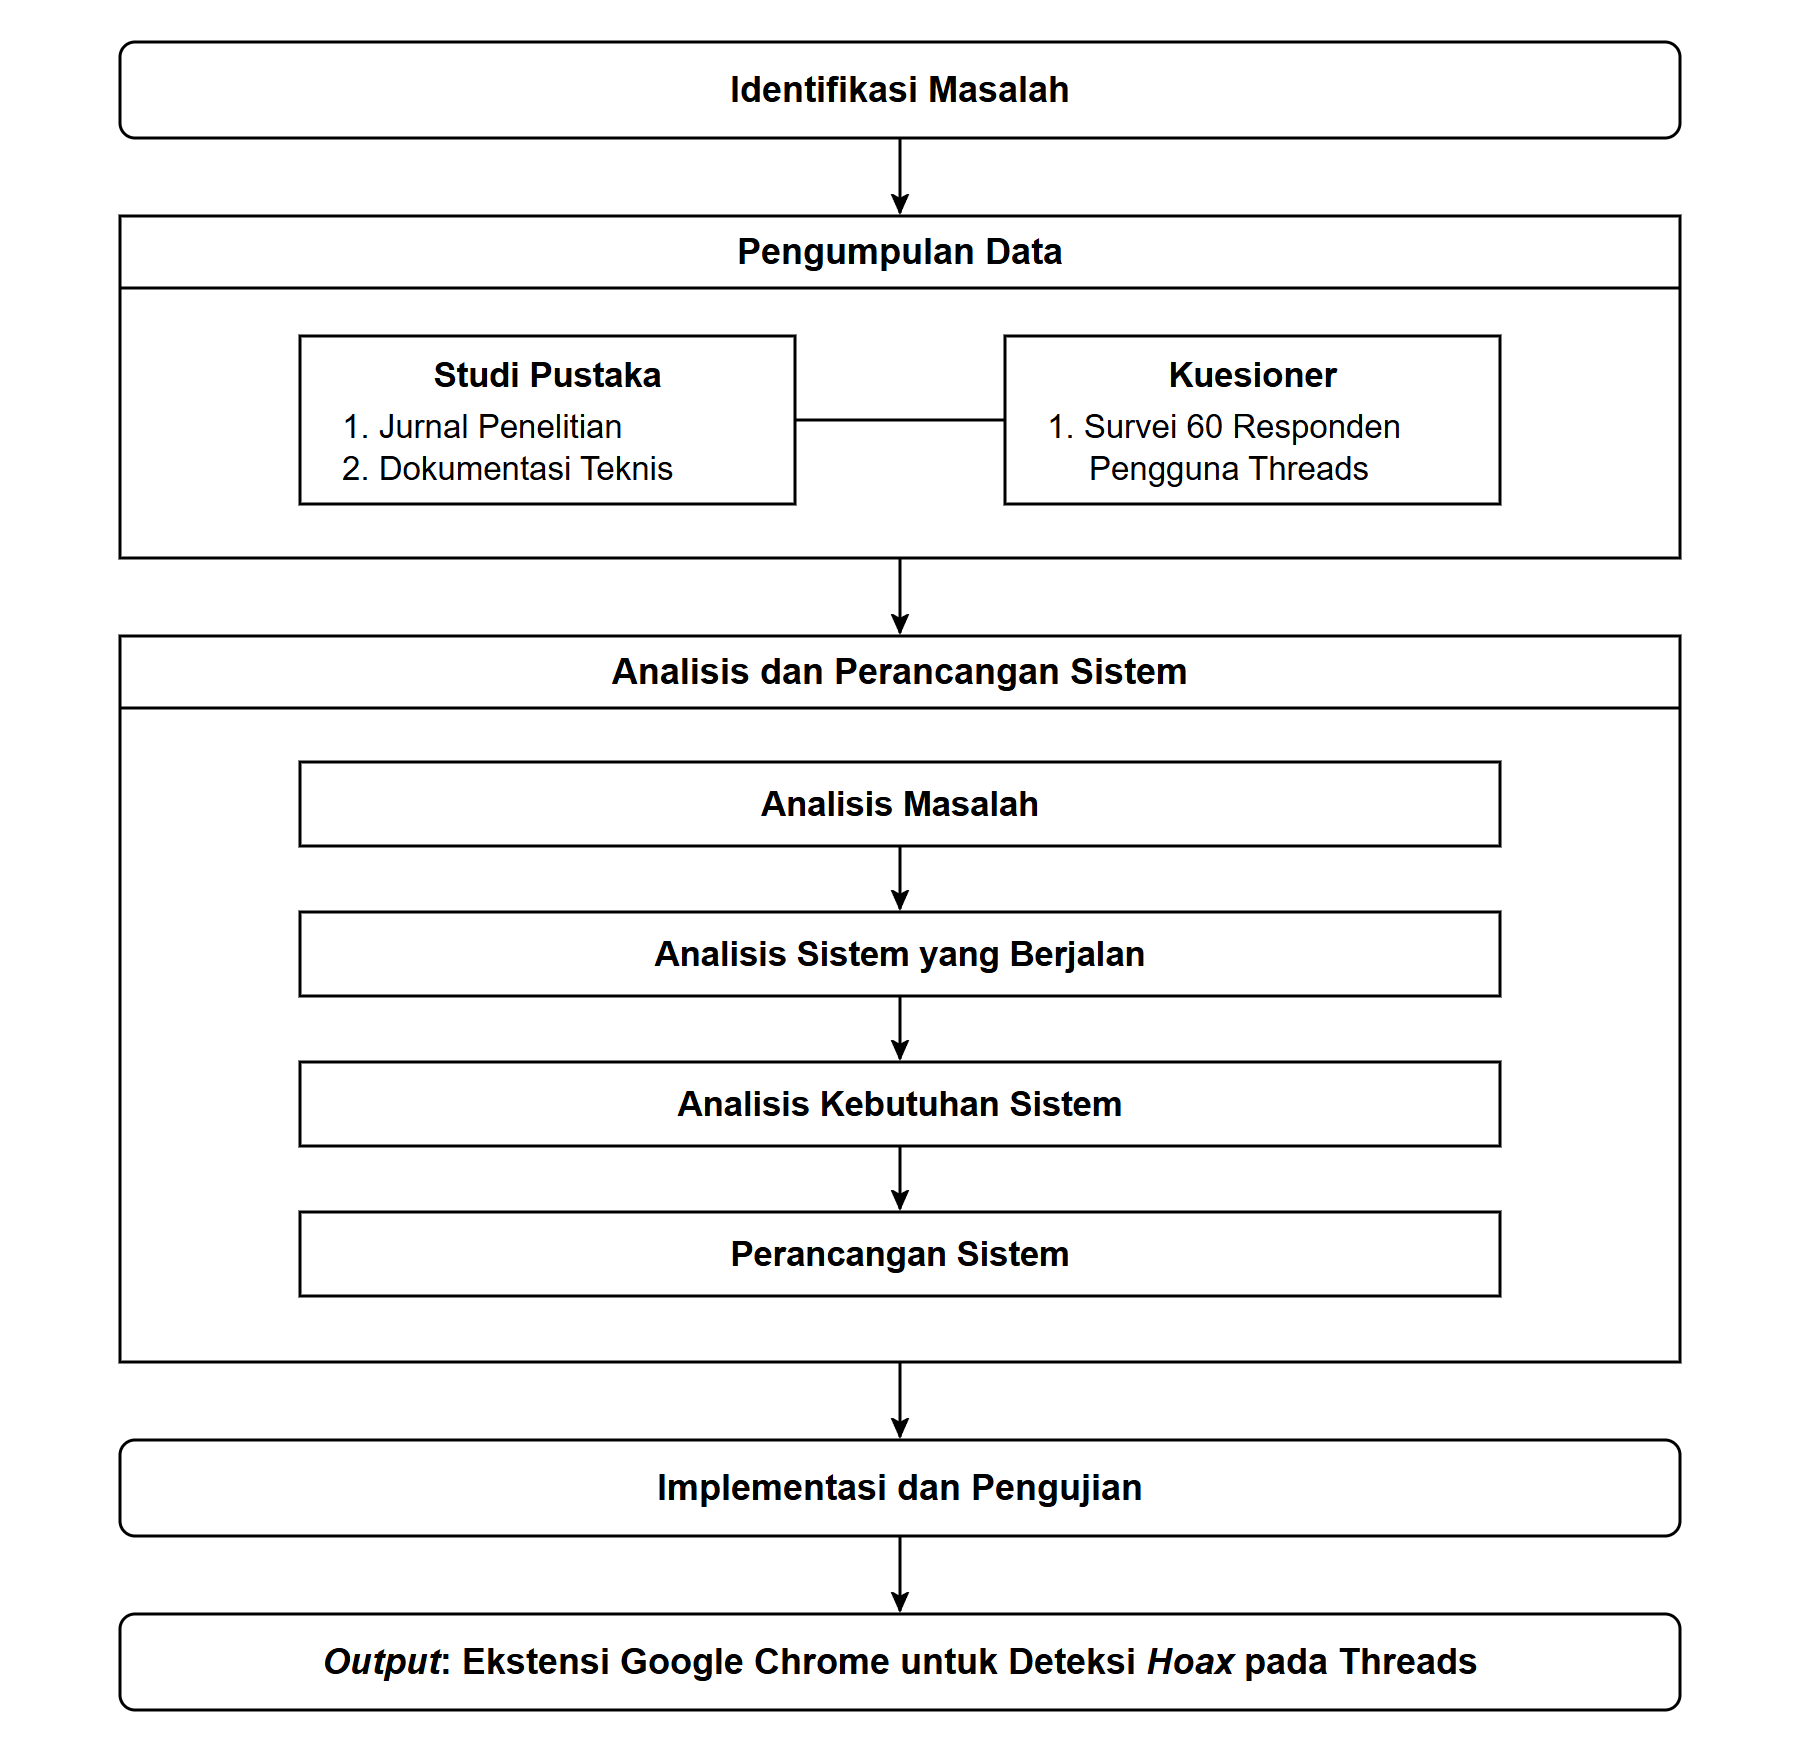
\includegraphics[width=0.92\textwidth]{gambar/metodologi_penelitian.png}
  \caption{Diagram alur metodologi penelitian}
  \label{fig:metodologi}
\end{figure}

Penjelasan mengenai masing-masing tahapan pada Gambar~\ref{fig:metodologi} diuraikan sebagai berikut:
\begin{enumerate}[leftmargin=1.27cm,itemsep=4pt,topsep=3pt]
  \item \tocsub{1.}{Identifikasi Masalah}\textbf{Identifikasi Masalah}\par
  \hspace*{1.27cm}Tahap awal penelitian dilakukan dengan mengamati fenomena penyebaran kabar bohong dan sindiran pada lini masa Threads versi \textit{web}, serta mengidentifikasi kendala yang dialami pengguna ketika harus memeriksa kebenaran informasi secara manual di luar halaman Threads.

  \item \tocsub{2.}{Pengumpulan Data}\textbf{Pengumpulan Data}\par
  \hspace*{1.27cm}Pengumpulan data dilakukan melalui dua kegiatan pendukung untuk memperkuat dasar perancangan sistem:
  \begin{enumerate}[label=\alph*.,leftmargin=0.7cm,itemsep=3pt,topsep=2pt]
    \item \tocsubsub{a.}{Studi Pustaka}\textbf{Studi Pustaka}\par
    \hspace*{1.27cm}Mempelajari artikel jurnal ilmiah dan dokumentasi resmi yang berkaitan dengan pemeriksaan fakta otomatis (\textit{automated fact-checking}), deteksi berita \textit{hoax} berbahasa Indonesia, arsitektur ekstensi Google Chrome \textit{Manifest V3}, serta otomasi \textit{browser} menggunakan Playwright.
    \item \tocsubsub{b.}{Kuesioner}\textbf{Kuesioner}\par
    \hspace*{1.27cm}Menyebarkan kuesioner kepada 60 responden pengguna Threads untuk memetakan kebiasaan responden saat menemukan informasi meragukan serta memastikan tingginya kebutuhan terhadap alat bantu pemeriksaan fakta yang terpasang langsung di \textit{browser}.
  \end{enumerate}

  \item \tocsub{3.}{Analisis dan Perancangan Sistem}\textbf{Analisis dan Perancangan Sistem}\par
  \hspace*{1.27cm}Tahap pengembangan perangkat lunak mengacu pada alur sistematis model \textit{Waterfall} yang pada bagian analisis dan perancangannya dibagi menjadi empat sub-tahap:
  \begin{enumerate}[label=3.\arabic*,leftmargin=0.9cm,itemsep=3pt,topsep=2pt]
    \item \tocsubsub{3.1}{Analisis Masalah}\textbf{Analisis Masalah}\par
    \hspace*{1.27cm}Menguraikan secara mendalam akar kendala teknis yang hendak diselesaikan, meliputi variasi penulisan teks dan kalimat sindiran di Threads, keterbatasan data statis terhadap isu baru, serta pencegahan rujukan berita yang tidak sesuai konteks.
    \item \tocsubsub{3.2}{Analisis Sistem yang Berjalan}\textbf{Analisis Sistem yang Berjalan}\par
    \hspace*{1.27cm}Memetakan alur kerja manual pengguna saat ini mulai dari menyalin teks unggahan di Threads hingga mencari klarifikasi sendiri di mesin pencari pada \textit{tab} terpisah.
    \item \tocsubsub{3.3}{Analisis Kebutuhan Sistem}\textbf{Analisis Kebutuhan Sistem}\par
    \hspace*{1.27cm}Menentukan daftar kebutuhan fungsional pada sisi ekstensi maupun sisi \textit{server} \textit{backend}, struktur elemen HTML/DOM halaman Threads yang perlu diekstraksi, serta spesifikasi perangkat keras dan perangkat lunak yang dibutuhkan.
    \item \tocsubsub{3.4}{Perancangan Sistem}\textbf{Perancangan Sistem}\par
    \hspace*{1.27cm}Merancang arsitektur komunikasi klien-\textit{server}, alur penelusuran fakta dua lapis (Google AI Overview dan Google News RSS), pemodelan visual menggunakan \textit{Unified Modeling Language} (UML) yang mencakup \textit{Use Case Diagram}, \textit{Activity Diagram}, dan \textit{Sequence Diagram}, serta perancangan tampilan lencana (\textit{badge}), \textit{tooltip}, dan jendela \textit{popup}.
  \end{enumerate}

  \item \tocsub{4.}{Implementasi dan Pengujian}\textbf{Implementasi dan Pengujian}\par
  \hspace*{1.27cm}Hasil perancangan diterjemahkan ke dalam kode program ekstensi Google Chrome (TypeScript dan React) serta layanan \textit{server} \textit{backend} (Node.js, Express.js, dan Playwright). Selanjutnya dilakukan pengujian fungsional dengan metode \textit{black-box testing} pada antarmuka ekstensi maupun REST API, diikuti pengujian kinerja klasifikasi pada sekumpulan klaim uji berbahasa Indonesia menggunakan \textit{confusion matrix} (akurasi, presisi, \textit{recall}, dan \textit{F1-score}) beserta evaluasi kesesuaian sumber rujukan dan waktu respons.

  \item \tocsub{5.}{\textit{Output}}\textbf{\textit{Output}}\par
  \hspace*{1.27cm}Tahap akhir menghasilkan luaran berupa perangkat lunak ekstensi Google Chrome pendeteksi indikasi \textit{hoax} berbasis teks pada platform Threads yang terintegrasi dengan \textit{server} penelusuran fakta \textit{real-time}, lengkap dengan laporan hasil pengujian fungsional dan evaluasi akurasinya.
\end{enumerate}

\section{Sistematika Penulisan}

Sistematika penulisan skripsi ini disusun ke dalam lima bab yang saling berkaitan guna memberikan gambaran utuh mengenai jalannya penelitian:

\noindent\textbf{BAB 1 PENDAHULUAN}\par
Menguraikan latar belakang masalah penyebaran informasi \textit{hoax} pada platform Threads, kondisi pemeriksaan manual berdasarkan fakta dan kuesioner 60 responden, akar permasalahan, pemilihan teknologi penelusuran \textit{real-time} dan ekstensi Chrome, identifikasi masalah, maksud dan tujuan, batasan masalah, metodologi penelitian, serta sistematika penulisan.

\noindent\textbf{BAB 2 TINJAUAN PUSTAKA}\par
Memaparkan landasan teori umum yang mendukung pembangunan sistem (konsep umum sistem, informasi, dan deteksi \textit{hoax}, klasifikasi \textit{hoax} dan \textit{satire}, struktur halaman \textit{web} Threads, arsitektur ekstensi Chrome \textit{Manifest V3}, \textit{server} \textit{backend}, serta penelusuran Google AI Overview dan Google News RSS), penjelasan metode penelitian (pengolahan kuesioner, \textit{system engineering}, \textit{system analysis}, metode pengembangan perangkat lunak \textit{Waterfall}, pemodelan UML, \textit{black-box testing}, dan \textit{confusion matrix}), perangkat lunak (\textit{tools}) yang digunakan termasuk \textit{Integrated Development Environment} (IDE) Google Antigravity, serta kajian penelitian terdahulu (\textit{state of the art}).

\noindent\textbf{BAB 3 METODE PENELITIAN}\par
Menjelaskan secara rinci tahapan analisis dan perancangan sistem, mencakup analisis masalah, analisis prosedur berjalan, analisis struktur DOM halaman Threads, spesifikasi kebutuhan fungsional dan non-fungsional, perancangan arsitektur dan alur penelusuran fakta, pemodelan UML, kontrak data API, serta rancangan antarmuka pengguna.

\noindent\textbf{BAB 4 HASIL DAN PEMBAHASAN}\par
Menyajikan hasil implementasi kode program dan antarmuka ekstensi Google Chrome beserta \textit{server} \textit{backend}, diikuti hasil pengujian fungsional \textit{black-box}, hasil pengukuran kinerja deteksi menggunakan \textit{confusion matrix}, evaluasi kesesuaian sumber berita rujukan, serta pembahasan mendalam atas temuan pengujian.

\noindent\textbf{BAB 5 KESIMPULAN DAN SARAN}\par
Berisi kesimpulan yang merangkum capaian penelitian dalam menjawab seluruh tujuan pada Bab 1 berdasarkan bukti hasil pengujian pada Bab 4, disertai saran pengembangan untuk penelitian berikutnya.

% ==============================================================================
% BAB 2 TINJAUAN PUSTAKA
% ==============================================================================
\babbaru{TINJAUAN PUSTAKA}

\section{Landasan Teori Umum}

Landasan teori umum pada bagian ini disusun selaras dengan permasalahan dan teknologi penyelesaian yang telah dirumuskan pada Bab 1, mulai dari konsep dasar sistem, informasi, dan karakteristik konten bermasalah di media sosial Threads hingga arsitektur ekstensi \textit{browser} dan penelusuran bukti \textit{web} secara \textit{real-time}.

\subsection{Sistem}

Secara umum, sistem merupakan sekumpulan elemen, komponen, atau prosedur yang saling terhubung dan berinteraksi secara teratur untuk mencapai suatu tujuan tertentu. Dalam bidang rekayasa perangkat lunak, sebuah sistem berbasis komputer bekerja dengan menerima masukan (\textit{input}) dari pengguna atau lingkungan luar, memproses masukan tersebut melalui serangkaian aturan logika yang terstruktur, serta menghasilkan keluaran (\textit{output}) yang dapat dimanfaatkan kembali oleh penggunanya. Keberhasilan suatu sistem sangat bergantung pada keselarasan kerja antar-komponen penyusunnya, sehingga apabila salah satu bagian mengalami hambatan maka kinerja sistem secara keseluruhan turut terpengaruh.

\subsection{Informasi}

Informasi adalah sekumpulan data mentah yang telah diolah, diklasifikasikan, dan diinterpretasikan ke dalam suatu konteks yang bermakna sehingga memiliki nilai guna bagi penerimanya dalam mengambil keputusan. Nilai dari suatu informasi ditentukan oleh tiga karakteristik utama, yaitu keakuratan (bebas dari kesalahan atau manipulasi fakta), ketepatan waktu (tersedia pada saat dibutuhkan), dan relevansi (sesuai dengan topik persoalan yang sedang dihadapi oleh pengguna). Di lingkungan digital yang terbuka, informasi yang belum teruji kebenarannya dapat memicu kesalahpahaman apabila langsung dijadikan dasar tindakan oleh pembaca.

\subsection{Deteksi \textit{Hoax}}

Deteksi \textit{hoax} merupakan proses pemeriksaan dan pengujian klaim informasi untuk membedakan antara pernyataan faktual yang terverifikasi dengan kabar bohong yang tidak memiliki dasar bukti yang sah. Dalam pendekatan komputasi modern, deteksi \textit{hoax} terotomasi (\textit{automated fact-checking}) dilakukan dengan mengekstraksi inti pernyataan dari suatu teks, menelusuri bukti pembanding dari sumber rujukan tepercaya, serta menyimpulkan tingkat kebenaran klaim tersebut disertai alasan dan tautan buktinya agar pengguna dapat menilai keabsahan informasi secara objektif.

\subsection{\textit{Hoax}}

\textit{Hoax} (kabar bohong) adalah informasi atau berita palsu yang tidak didasarkan pada kenyataan, namun dirangkai sedemikian rupa menggunakan kalimat yang provokatif atau meyakinkan agar dianggap sebagai peristiwa nyata oleh masyarakat. Penyebaran \textit{hoax} di media sosial umumnya memanfaatkan judul sensasional, pencatutan nama tokoh atau instansi resmi, serta klaim darurat yang memancing reaksi emosional pembaca untuk segera membagikannya kembali tanpa memeriksa sumber aslinya.

\subsection{Misinformasi}

Misinformasi (\textit{misinformation}) adalah informasi tidak akurat atau keliru yang disebarkan oleh pengguna tanpa adanya niat jahat untuk menipu orang lain. Kondisi ini sering terjadi ketika pengguna media sosial salah menafsirkan isi berita, mempercayai kabar lama yang diunggah ulang seolah-olah baru terjadi, atau terburu-buru meneruskan pesan berantai kepada rekan-rekannya karena mengira informasi tersebut bermanfaat.

\subsection{Disinformasi}

Disinformasi (\textit{disinformation}) merupakan informasi palsu yang secara sadar dan sengaja direkayasa serta disebarkan untuk menyesatkan publik, menggiring opini masyarakat, merugikan reputasi pihak tertentu, atau memperoleh keuntungan finansial secara tidak sah. Contoh disinformasi yang marak ditemukan di media sosial meliputi pengumuman pendaftaran bantuan pemerintah palsu, rekayasa kutipan pernyataan pejabat publik, hingga penyebaran kabar krisis palsu.

\subsection{\textit{Satire}}

\textit{Satire} atau sindiran (\textit{satire/parody}) adalah gaya penyampaian pesan yang menggunakan perumpamaan berlebihan, ironi, plesetan nama lembaga, atau cerita rekaan sebagai sarana humor maupun kritik sosial. Meskipun pembuat unggahan \textit{satire} tidak berniat menipu pembaca, pengguna media sosial yang tidak memahami latar belakang candaan tersebut sering kali menganggap isi kalimatnya sebagai kejadian sungguhan. Oleh sebab itu, sistem pemeriksa fakta pada media sosial perlu mengenali konteks sindiran agar dapat memberi tahu pengguna bahwa unggahan tersebut bukan merupakan klaim berita faktual.

\subsection{Platform Media Sosial Threads}

Threads merupakan layanan jejaring sosial mikroblog berbasis teks yang dikembangkan oleh Meta Platforms dan dapat diakses melalui \textit{browser} komputer pada alamat \texttt{https://www.threads.com}. Berbeda dengan Instagram yang berfokus pada berbagi foto dan video, Threads dirancang khusus untuk percakapan publik melalui unggahan teks singkat hingga 500 karakter per bagian utas (\textit{thread}). Karakteristik unggahan yang ringkas dan menyebar cepat melalui algoritma rekomendasi menjadikan Threads banyak digunakan untuk mendiskusikan berita terkini, namun hingga saat ini antarmuka halaman \textit{web} Threads belum menyediakan fitur pemeriksa fakta bawaan pada setiap kartu unggahan.

\subsection{\textit{Document Object Model} (DOM)}

\textit{Document Object Model} (DOM) adalah antarmuka pemrograman standar bagi dokumen HTML yang merepresentasikan seluruh elemen halaman \textit{web} ke dalam struktur pohon objek (\textit{tree structure}) sehingga isi, struktur, dan tampilannya dapat dibaca maupun dimodifikasi secara dinamis menggunakan JavaScript. Pada halaman \textit{web} Threads yang berjalan sebagai \textit{Single-Page Application} (SPA), daftar unggahan baru dimuat secara terus-menerus ketika pengguna menggulir layar dan nama kelas tampilannya (\textit{CSS class}) diacak saat proses kompilasi. Oleh karena itu, pembacaan data unggahan oleh ekstensi \textit{browser} harus menargetkan struktur simpul DOM yang stabil seperti elemen \texttt{article}, atribut \texttt{data-pressable-container}, tautan akun \texttt{/@username}, elemen waktu \texttt{<time datetime="...">}, serta blok teks beratribut \texttt{dir="auto"}.

\subsection{Ekstensi \textit{Browser} Google Chrome \textit{Manifest V3}}

Ekstensi Google Chrome adalah perangkat lunak tambahan berbasis teknologi \textit{web} (HTML, CSS, dan JavaScript/TypeScript) yang dipasang pada \textit{browser} Google Chrome untuk menambahkan fitur khusus dan berinteraksi langsung dengan halaman situs yang sedang dibuka pengguna. Spesifikasi terbaru yang ditetapkan oleh Google adalah \textit{Manifest V3}, yang menggantikan halaman latar belakang terus-menerus (\textit{persistent background page}) dengan \textit{Service Worker} berbasis kejadian (\textit{event-driven}) guna menghemat penggunaan memori serta meningkatkan keamanan izin akses domain.

Dalam sistem deteksi \textit{hoax} berarsitektur klien-\textit{server} yang dirancang pada penelitian ini, komunikasi antara komponen internal ekstensi Chrome \textit{Manifest V3}, layanan \textit{server} \textit{backend}, dan sumber pencarian \textit{web} berjalan sebagaimana digambarkan pada Gambar~\ref{fig:arsitektur}.

\begin{figure}[htbp]
  \centering
  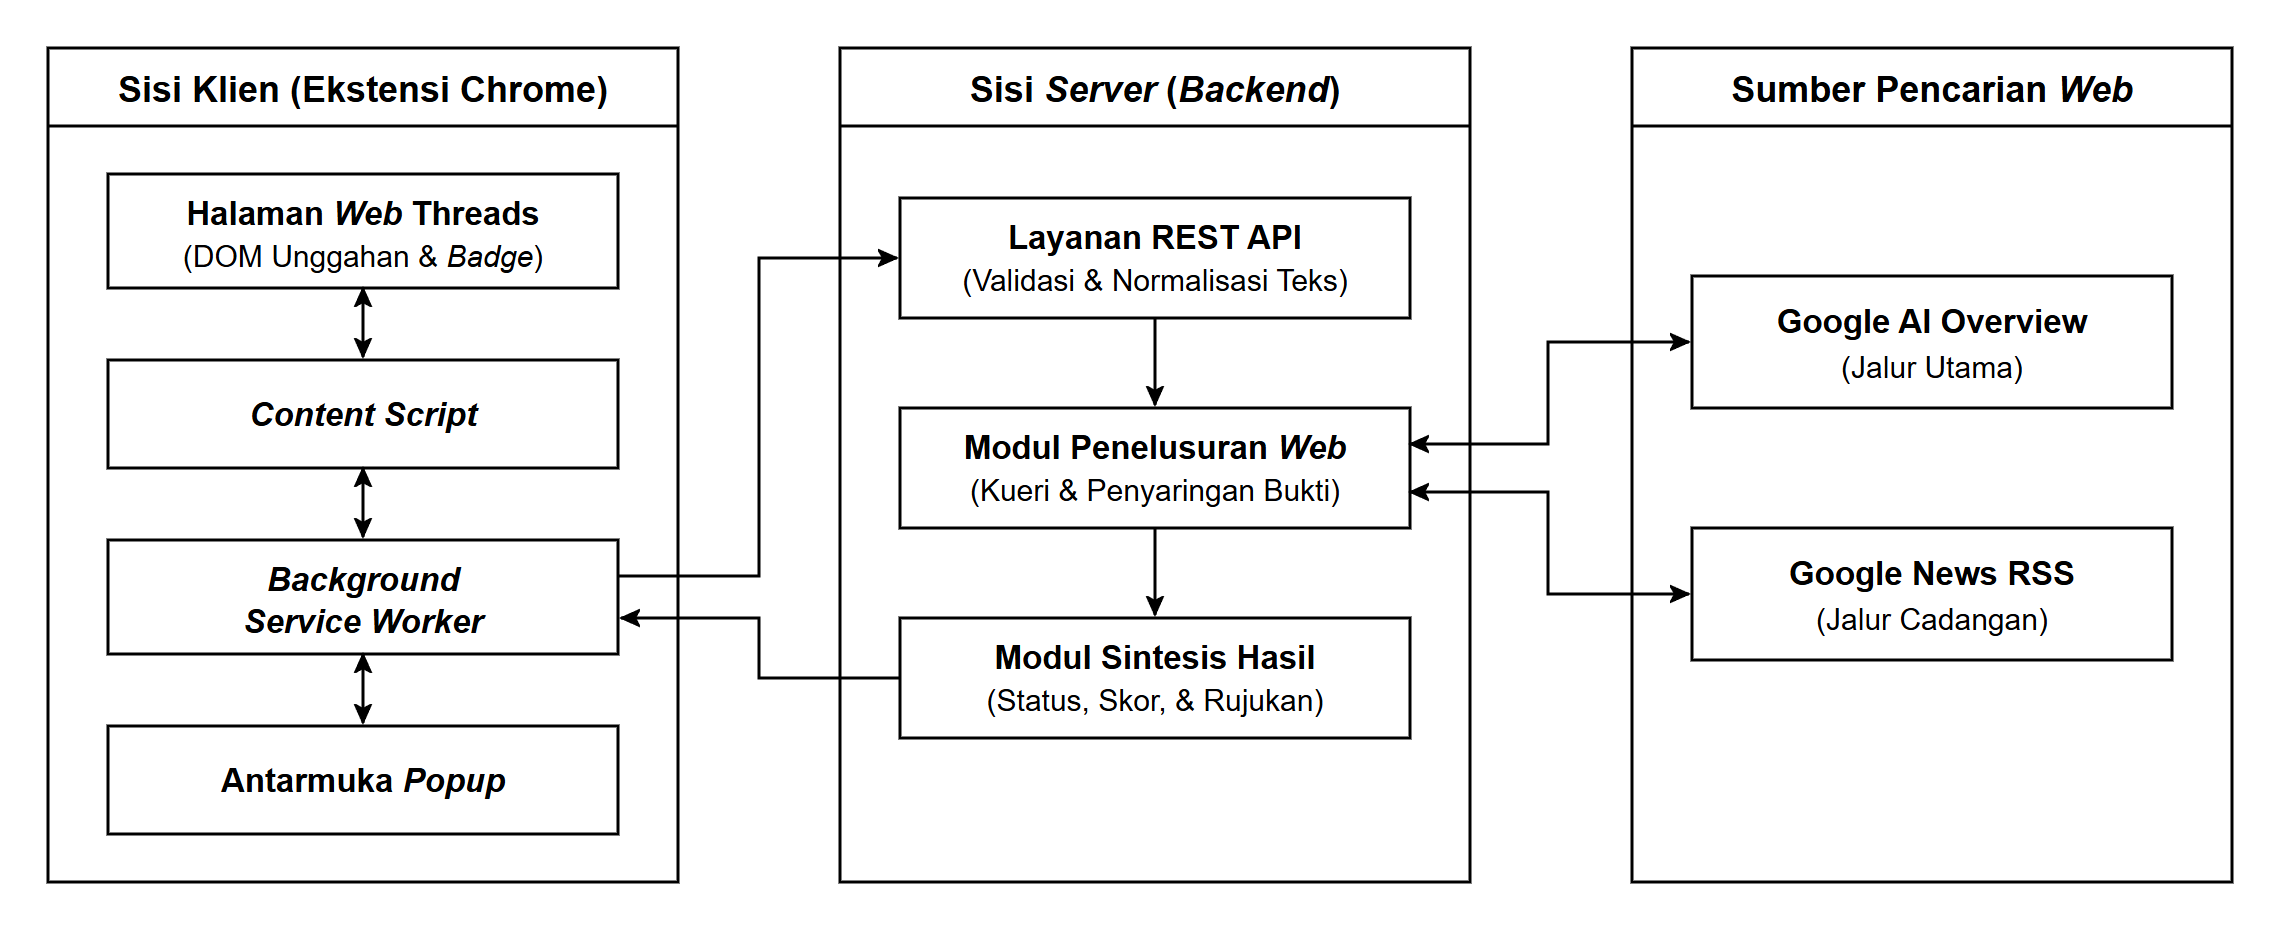
\includegraphics[width=0.96\textwidth]{gambar/arsitektur_umum.png}
  \caption{Arsitektur komunikasi ekstensi Chrome dan \textit{server} \textit{backend}}
  \label{fig:arsitektur}
\end{figure}

Berdasarkan Gambar~\ref{fig:arsitektur}, arsitektur sisi klien pada ekstensi Google Chrome dibagi menjadi tiga bagian yang memiliki peran terpisah namun saling bertukar pesan:
\begin{enumerate}[leftmargin=0.8cm,itemsep=3pt,topsep=2pt]
  \item \textit{Content Script}: Skrip yang disisipkan langsung ke halaman \textit{web} Threads untuk mendeteksi elemen unggahan yang diklik kanan oleh pengguna, mengekstraksi teks beserta identitas akun dari DOM, serta menyuntikkan elemen visual berupa lencana (\textit{badge}) status dan jendela keterangan (\textit{tooltip}) hasil pemeriksaan.
  \item \textit{Background Service Worker}: Pengendali di balik layar yang mendaftarkan menu klik kanan (\texttt{contextMenus}), meneruskan data unggahan ke \textit{server} \textit{backend} melalui permintaan HTTP, menyimpan riwayat pemeriksaan ke penyimpanan lokal \textit{browser} (\texttt{chrome.storage.local}), dan mengirim balik hasil analisis ke \textit{Content Script}.
  \item Antarmuka \textit{Popup}: Jendela ringkas yang muncul ketika pengguna menekan ikon ekstensi pada bilah alat \textit{browser} untuk menampilkan ringkasan statistik pemeriksaan, daftar riwayat klaim yang pernah diperiksa, serta pengaturan tampilan.
\end{enumerate}

\subsection{Layanan \textit{Server} \textit{Backend}}

Layanan \textit{server} \textit{backend} merupakan komponen perangkat lunak di sisi peladen yang bertugas menangani logika pemrosesan data, menjalankan otomasi penelusuran bukti ke mesin pencari, serta menyusun kesimpulan analisis di luar lingkungan \textit{tab} \textit{browser} pengguna. Pemisahan proses penelusuran fakta ke dalam \textit{server} \textit{backend} tersendiri bertujuan agar kinerja \textit{browser} pengguna tetap ringan saat menjelajahi Threads dan proses pengambilan data dari berbagai situs berita tidak terhalang oleh pembatasan keamanan lintas domain (\textit{Cross-Origin Resource Sharing}/CORS).

\subsection{REST API}

\textit{Representational State Transfer Application Programming Interface} (REST API) adalah standar arsitektur komunikasi jaringan yang memungkinkan pertukaran data antara aplikasi klien (ekstensi \textit{browser}) dan aplikasi \textit{server} melalui protokol HTTP menggunakan metode standar seperti \texttt{GET}, \texttt{POST}, dan \texttt{DELETE}. Dalam sistem ini, REST API menggunakan format pertukaran data \textit{JavaScript Object Notation} (JSON) yang ringan dan terstruktur untuk mengirimkan teks unggahan yang akan diperiksa serta mengembalikan hasil analisis beserta daftar tautan sumber rujukan ke ekstensi.

\subsection{Normalisasi Teks \textit{Unicode}}

Normalisasi teks \textit{Unicode} adalah proses transformasi deretan karakter ke dalam bentuk kode standar yang seragam sebelum teks diolah oleh algoritma pencarian maupun pencocokan kata kunci. Banyak unggahan viral di media sosial menggunakan huruf dekoratif atau huruf tebal matematika \textit{Unicode} agar tampak mencolok di lini masa. Melalui standar \textit{Normalization Form Compatibility Composition} (NFKC), seluruh karakter bergaya khusus tersebut diuraikan lalu disusun kembali menjadi huruf alfabet ASCII standar sehingga kalimat klaim dapat dibaca secara utuh oleh mesin pencari.

\subsection{Penelusuran Bukti Fakta \textit{Real-Time}}

Penelusuran bukti fakta \textit{real-time} (\textit{real-time web retrieval}) adalah pendekatan verifikasi klaim yang mengambil bukti langsung dari indeks mesin pencari dan portal berita daring pada saat permintaan pemeriksaan diterima. Pendekatan ini menggabungkan ekstraksi Google AI Overview (Ringkasan AI) menggunakan otomasi \textit{browser} tanpa tampilan (\textit{headless browser}) serta penelusuran umpan berita Google News RSS sebagai jalur cadangan. Dengan mengambil bukti secara langsung dari \textit{web}, sistem dapat memeriksa kebenaran peristiwa atau isu viral yang baru saja terjadi pada hari yang sama tanpa bergantung pada pelatihan ulang \textit{dataset} statis.

\subsection{Pencegahan Halusinasi Rujukan}

Halusinasi rujukan merupakan kondisi ketika suatu sistem kecerdasan buatan menghasilkan tautan berita fiktif atau menyertakan artikel rujukan yang sebenarnya membahas topik lain di luar isi klaim yang sedang diperiksa. Untuk mencegah hal tersebut, setiap kandidat tautan rujukan yang diperoleh dari mesin pencari harus melewati proses resolusi alamat URL asli dan penyaringan kesesuaian konteks menggunakan pencocokan irisan kata kunci klaim serta kata kunci peristiwa. Hanya artikel berita yang memiliki keterkaitan langsung dengan pokok bahasan unggahan yang disertakan sebagai bukti pendukung pada hasil akhir.

\section{Metode Penelitian}

Uraian metode pada bagian ini menjadi landasan teoretis bagi tahapan metodologi penelitian yang telah digambarkan pada Subbab 1.5, meliputi kuesioner, rekayasa sistem (\textit{system engineering}), analisis sistem (\textit{system analysis}), model pengembangan perangkat lunak \textit{Waterfall}, pemodelan \textit{Unified Modeling Language} (UML), pengujian \textit{black-box}, serta evaluasi \textit{confusion matrix}.

\subsection{Kuesioner}

Kuesioner merupakan teknik pengumpulan data yang dilakukan dengan memberikan seperangkat pertanyaan tertulis kepada responden untuk memperoleh informasi mengenai pengalaman, kebiasaan, serta kebutuhan pengguna terhadap sistem yang akan dibangun. Dalam penelitian ini, kuesioner disebarkan kepada 60 responden pengguna Threads, kemudian data jawaban dari setiap butir pertanyaan tertutup diolah menggunakan perhitungan distribusi persentase deskriptif sebagaimana dituliskan pada Persamaan~(II.1):

\begin{equation}
  P = \frac{f}{N} \times 100\%
  \tag{II.1}
\end{equation}

dengan keterangan $P$ menyatakan nilai persentase untuk suatu pilihan jawaban (\%), $f$ menyatakan frekuensi atau banyaknya responden yang memilih jawaban tersebut, dan $N$ menyatakan jumlah seluruh responden kuesioner ($N = 60$).

\subsection{\textit{System Engineering} (Rekayasa Sistem)}

\textit{System engineering} (rekayasa sistem) merupakan tahapan tingkat sistem yang bertujuan menetapkan hubungan timbal balik antara perangkat lunak yang akan dibangun dengan seluruh elemen pembentuk sistem lainnya, meliputi perangkat keras (\textit{hardware}), perangkat lunak (\textit{software}), pengguna (\textit{brainware}), serta data dan jaringan komunikasi (\textit{data and network}). Karena perangkat lunak ekstensi \textit{browser} tidak berdiri sendiri melainkan beroperasi di dalam lingkungan halaman \textit{web} dan berkomunikasi dengan \textit{server} eksternal, perumusan batas sistem pada tahap \textit{system engineering} sangat penting agar seluruh komponen dapat bekerja secara selaras sebagaimana ditunjukkan pada Gambar~\ref{fig:syseng}.

\begin{figure}[htbp]
  \centering
  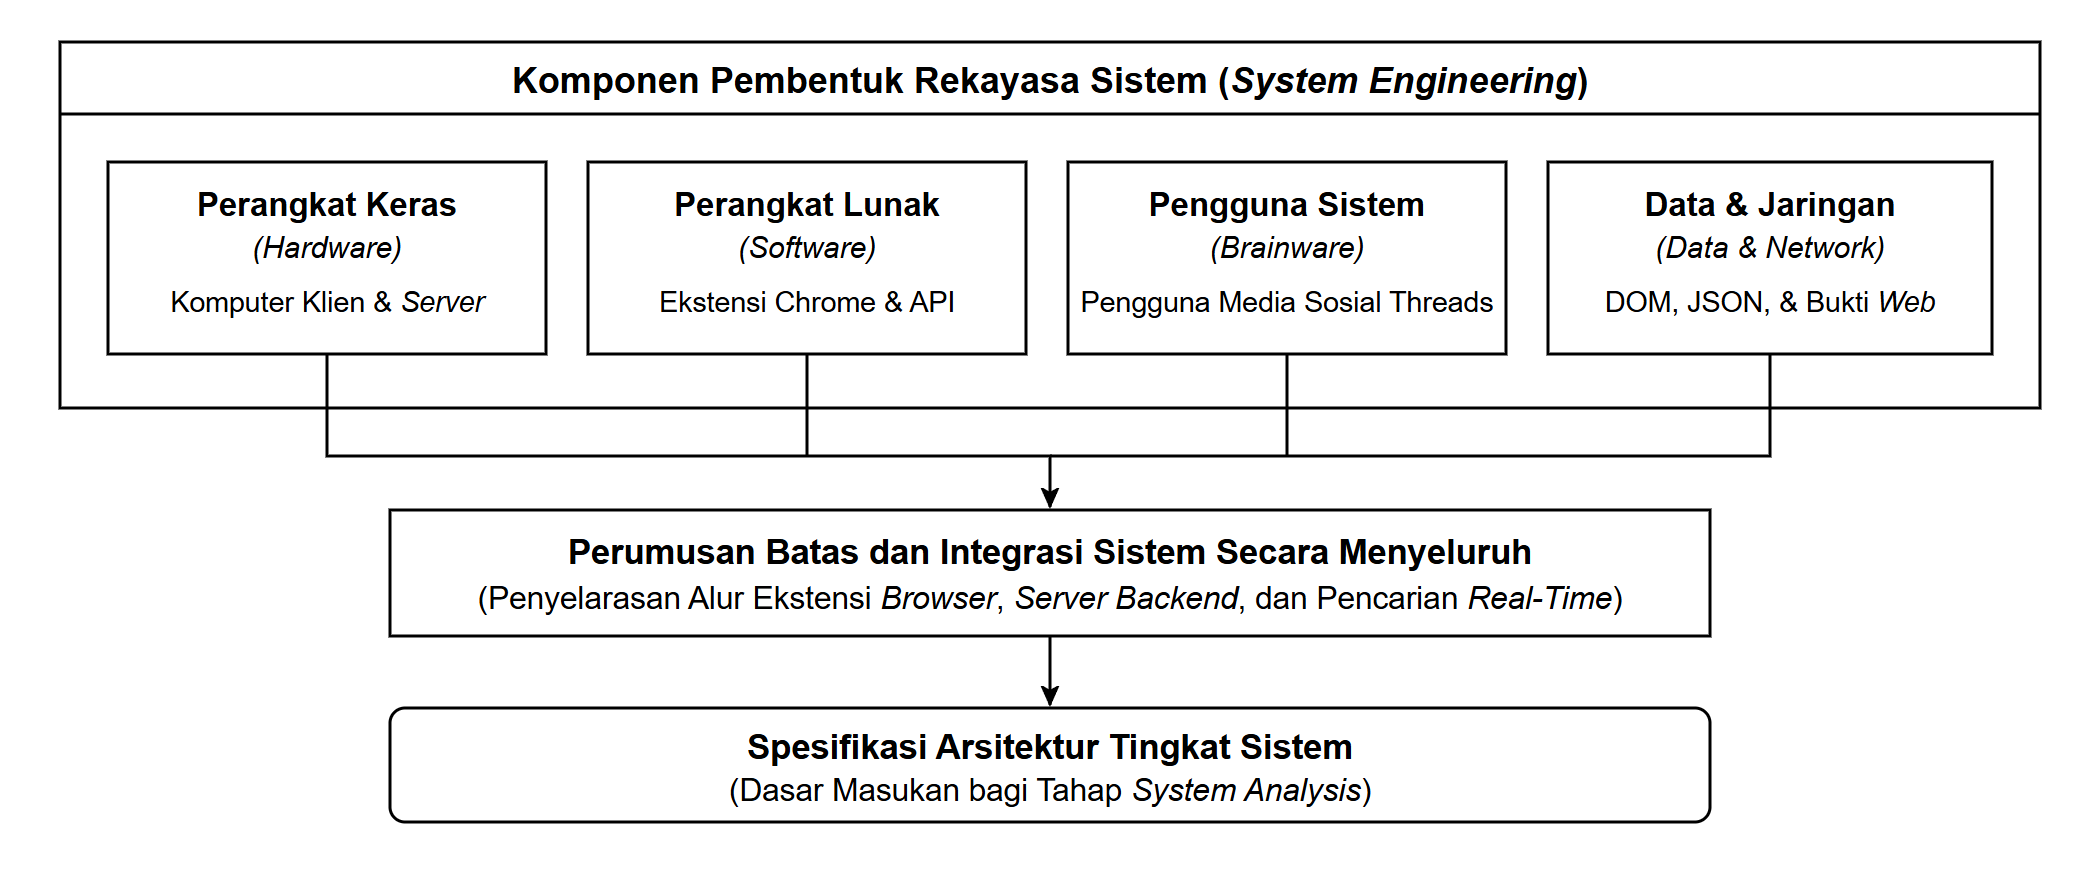
\includegraphics[width=0.94\textwidth]{gambar/system_engineering.png}
  \caption{Diagram alur \textit{system engineering} pada pengembangan sistem}
  \label{fig:syseng}
\end{figure}

Berdasarkan Gambar~\ref{fig:syseng}, tahap \textit{system engineering} menyatukan empat elemen utama, yaitu perangkat keras komputer klien dan \textit{server}, perangkat lunak ekstensi Chrome dan layanan REST API, pengguna media sosial Threads sebagai aktor pemicu verifikasi, serta aliran data DOM, objek JSON, dan bukti pencarian \textit{web} menjadi satu spesifikasi arsitektur tingkat sistem yang siap dianalisis lebih lanjut.

\subsection{\textit{System Analysis} (Analisis Sistem)}

\textit{System analysis} (analisis sistem) adalah proses penguraian suatu sistem secara menyeluruh ke dalam bagian-bagian komponennya dengan tujuan mengidentifikasi permasalahan yang terjadi, memahami karakteristik sistem yang sedang berjalan, serta merumuskan kebutuhan fungsional dan non-fungsional secara tepat sebelum tahap perancangan dimulai. Alur tahapan \textit{system analysis} yang diterapkan pada penelitian ini mengikuti empat langkah sistematis sebagaimana digambarkan pada Gambar~\ref{fig:sysana}.

\begin{figure}[htbp]
  \centering
  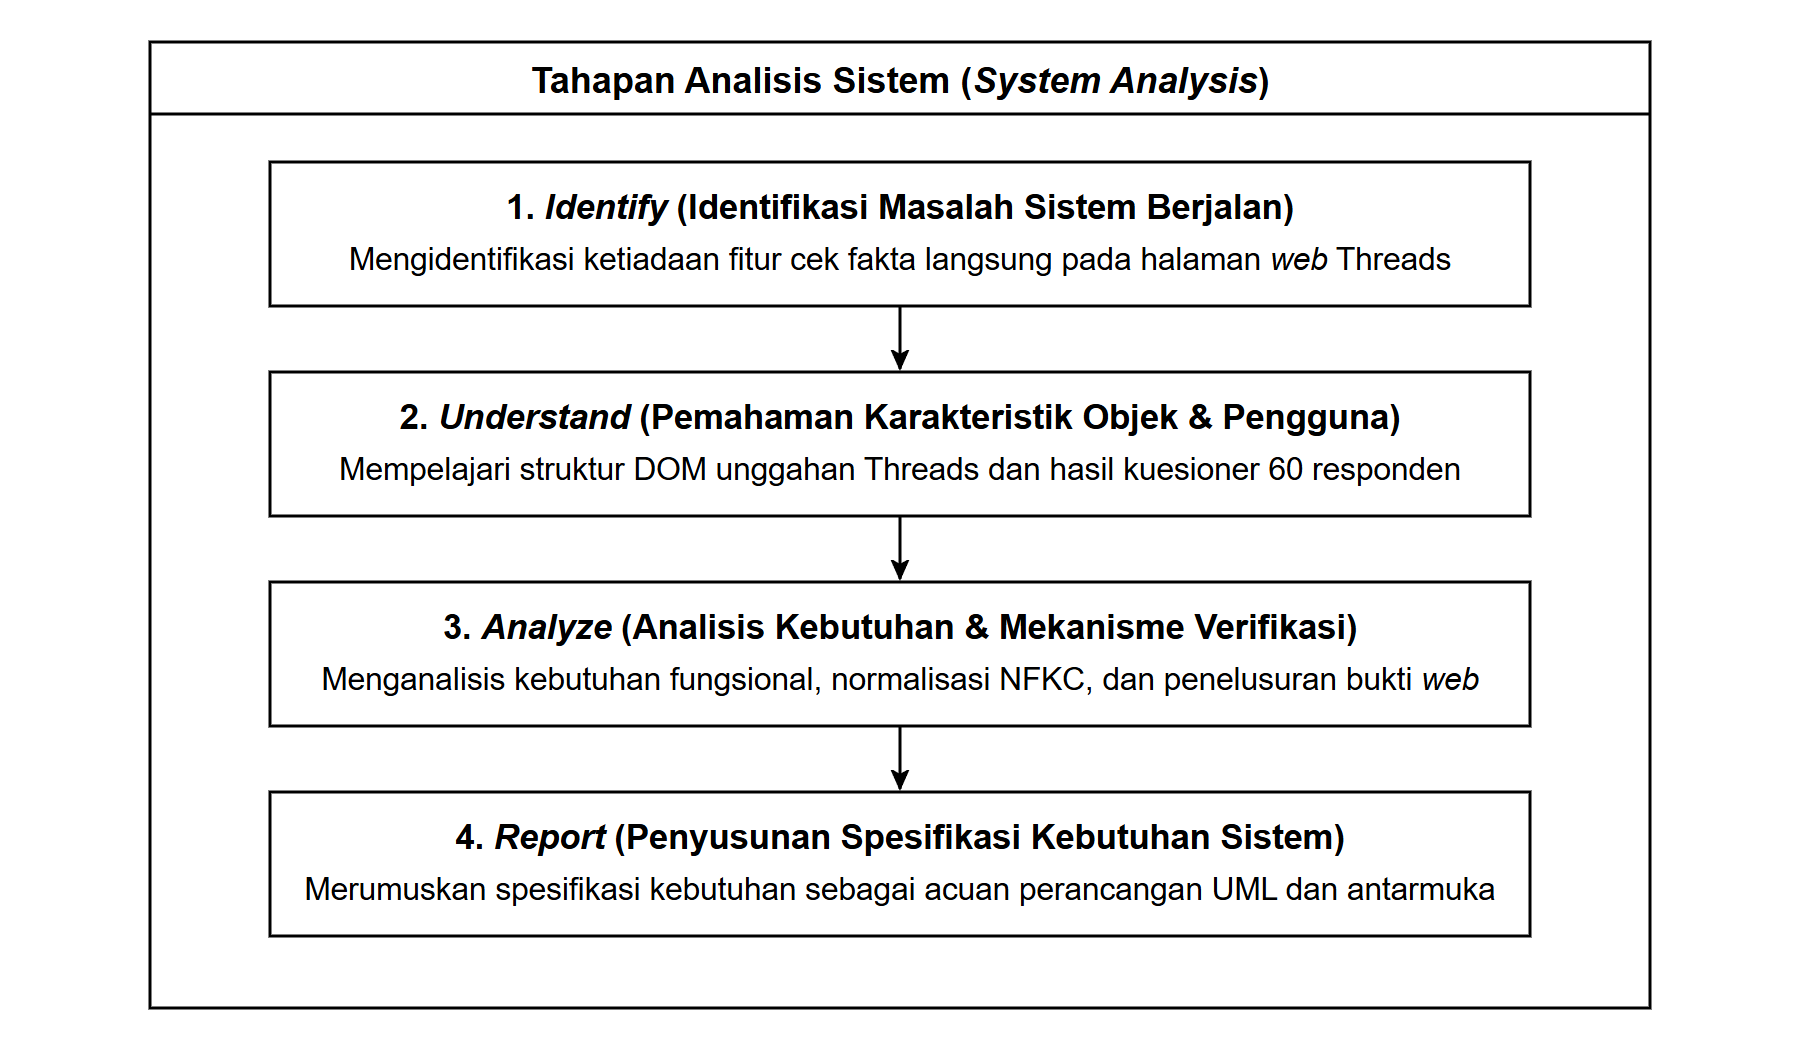
\includegraphics[width=0.88\textwidth]{gambar/system_analysis.png}
  \caption{Diagram tahapan \textit{system analysis} pada penelitian}
  \label{fig:sysana}
\end{figure}

Berdasarkan Gambar~\ref{fig:sysana}, keempat tahapan \textit{system analysis} dalam penelitian ini meliputi:
\begin{enumerate}[leftmargin=0.8cm,itemsep=2pt,topsep=2pt]
  \item \textit{Identify} (Identifikasi Masalah): Mengidentifikasi akar permasalahan pada sistem yang berjalan saat ini, yaitu ketiadaan fitur pemeriksaan fakta langsung pada halaman \textit{web} Threads sehingga pengguna harus memeriksa klaim secara manual di luar \textit{tab} \textit{browser}.
  \item \textit{Understand} (Pemahaman Karakteristik Objek dan Pengguna): Mempelajari struktur elemen DOM unggahan pada halaman \textit{web} Threads serta memahami kebutuhan pengguna berdasarkan hasil kuesioner terhadap 60 responden.
  \item \textit{Analyze} (Analisis Kebutuhan dan Mekanisme Verifikasi): Menganalisis daftar kebutuhan fungsional dan non-fungsional, aturan normalisasi teks \textit{Unicode} bentuk NFKC, serta alur ekstraksi bukti \textit{real-time} dari Google AI Overview dan Google News RSS.
  \item \textit{Report} (Penyusunan Spesifikasi Kebutuhan Sistem): Merangkum seluruh temuan analisis menjadi spesifikasi kebutuhan sistem yang terstruktur sebagai acuan langsung pada tahap perancangan UML dan antarmuka.
\end{enumerate}

\subsection{Metode Pengembangan Perangkat Lunak \textit{Waterfall}}

Proses rekayasa perangkat lunak dalam penelitian ini mengikuti model \textit{Waterfall} yang dikemukakan oleh Pressman dan Maxim. Model \textit{Waterfall} dipilih karena spesifikasi masalah, batasan fitur ekstensi, serta alur komunikasi antara \textit{browser} dan \textit{server} telah terdefinisi dengan jelas sejak awal penelitian, sehingga pengerjaan dapat dilakukan secara runtut dari tahap \textit{system engineering} dan \textit{system analysis} hingga tahap pemeliharaan sebagaimana ditunjukkan pada Gambar~\ref{fig:waterfall}.

\begin{figure}[htbp]
  \centering
  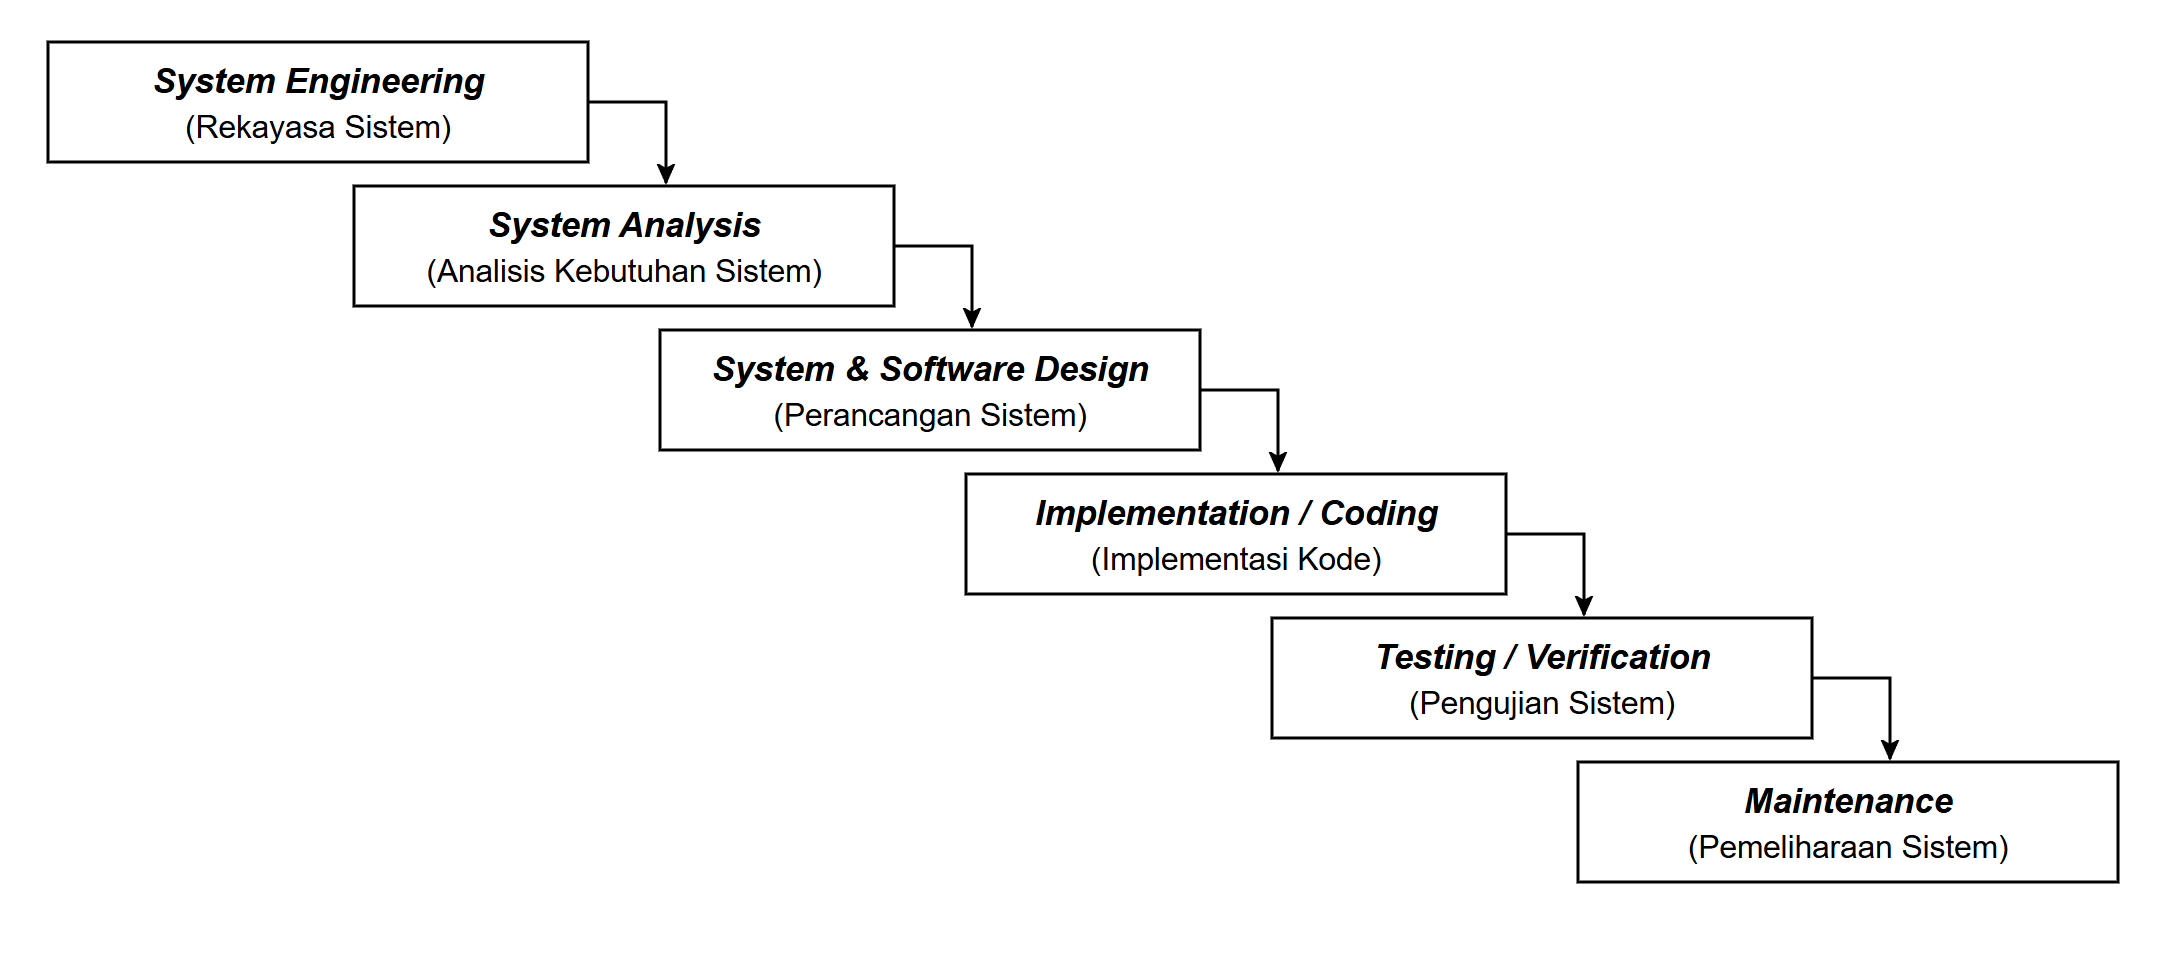
\includegraphics[width=0.92\textwidth]{gambar/metode_waterfall.png}
  \caption{Tahapan metode pengembangan perangkat lunak \textit{Waterfall}}
  \label{fig:waterfall}
\end{figure}

Keenam tahapan pada Gambar~\ref{fig:waterfall} memiliki keterkaitan langsung dengan langkah kerja penelitian pada Bab 1, yaitu:
\begin{enumerate}[leftmargin=0.8cm,itemsep=2pt,topsep=2pt]
  \item \textit{System Engineering} (Rekayasa Sistem): Menetapkan batas sistem secara menyeluruh serta menyelaraskan hubungan antara ekstensi \textit{browser} pada sisi klien, layanan \textit{server} \textit{backend}, pengguna Threads, dan sumber pencarian \textit{web}.
  \item \textit{System Analysis} (Analisis Kebutuhan Sistem): Mengumpulkan dan menganalisis kebutuhan fungsional serta non-fungsional perangkat lunak berdasarkan identifikasi masalah, pengamatan struktur DOM halaman Threads, dan hasil kuesioner pengguna.
  \item \textit{System and Software Design} (Perancangan Sistem): Menyusun arsitektur sistem tiga lapis, rancangan alur penelusuran dan penyaringan rujukan, diagram UML, struktur pertukaran data JSON, serta rancangan tampilan antarmuka.
  \item \textit{Implementation / Coding} (Implementasi Kode): Menerjemahkan seluruh rancangan ke dalam kode sumber ekstensi Chrome \textit{Manifest V3} dan layanan \textit{server} \textit{backend}.
  \item \textit{Testing / Verification} (Pengujian Sistem): Memeriksa kesesuaian seluruh fungsi sistem menggunakan pengujian \textit{black-box} serta mengukur ketepatan deteksi klaim uji menggunakan \textit{confusion matrix}.
  \item \textit{Maintenance} (Pemeliharaan Sistem): Mengevaluasi temuan batas hasil pengujian dan menyiapkan penyesuaian apabila terjadi perubahan struktur tampilan pada halaman \textit{web} Threads maupun halaman pencarian Google.
\end{enumerate}

\subsection{\textit{Unified Modeling Language} (UML)}

\textit{Unified Modeling Language} (UML) adalah bahasa pemodelan visual standar yang digunakan dalam rekayasa perangkat lunak berbasis objek untuk memvisualisasikan, merancang, dan mendokumentasikan alur kerja serta struktur sistem sebelum penulisan kode program dilakukan. Tiga jenis diagram UML yang digunakan dalam perancangan sistem ini meliputi:
\begin{enumerate}[leftmargin=0.8cm,itemsep=2pt,topsep=2pt]
  \item \textit{Use Case Diagram}: Menggambarkan daftar fungsi utama yang disediakan oleh ekstensi \textit{browser} serta interaksi antara aktor pengguna Threads dan sistem.
  \item \textit{Activity Diagram}: Memetakan urutan aktivitas kerja dari awal hingga akhir lintas komponen (\textit{swimlane}), mulai dari tindakan klik kanan pengguna pada unggahan hingga lencana hasil tampil di layar.
  \item \textit{Sequence Diagram}: Menjelaskan urutan waktu pertukaran pesan (\textit{message passing}) secara rinci antara \textit{Content Script}, \textit{Background Service Worker}, REST API pada \textit{server} \textit{backend}, dan modul penelusuran \textit{web}.
\end{enumerate}

\subsection{Pengujian \textit{Black-Box}}

Pengujian \textit{black-box} (\textit{black-box testing}) adalah metode pengujian perangkat lunak yang berfokus pada pemeriksaan kesesuaian fungsi masukan (\textit{input}) dan keluaran (\textit{output}) berdasarkan spesifikasi kebutuhan fungsional tanpa menguji struktur kode internal secara langsung. Dalam penelitian ini, pengujian \textit{black-box} digunakan untuk memverifikasi keberhasilan pembacaan unggahan pada DOM halaman Threads, penyuntikan lencana status dan \textit{tooltip} bukti rujukan, fungsi jendela \textit{popup} riwayat pemeriksaan, serta validasi respons \textit{endpoint} REST API pada \textit{server} \textit{backend}.

\subsection{\textit{Confusion Matrix}}

\textit{Confusion matrix} adalah tabel evaluasi kinerja klasifikasi yang membandingkan hasil prediksi sistem terhadap label kebenaran aktual (\textit{ground truth}) pada sekumpulan data uji. Dalam penelitian ini, \textit{confusion matrix} digunakan untuk mengukur ketepatan sistem dalam membedakan unggahan yang berindikasi \textit{hoax}/\textit{satire} (kelas positif) dan unggahan fakta yang valid (kelas negatif). Empat komponen utama pada \textit{confusion matrix} terdiri atas:
\begin{itemize}[leftmargin=0.8cm,itemsep=2pt,topsep=2pt]
  \item \textit{True Positive} (TP): Jumlah unggahan \textit{hoax}/\textit{satire} yang berhasil dideteksi dengan tepat sebagai terindikasi \textit{hoax}.
  \item \textit{True Negative} (TN): Jumlah unggahan fakta/valid yang berhasil dikenali dengan tepat sebagai terverifikasi benar.
  \item \textit{False Positive} (FP): Jumlah unggahan fakta/valid yang keliru ditandai sebagai \textit{hoax} oleh sistem.
  \item \textit{False Negative} (FN): Jumlah unggahan \textit{hoax}/\textit{satire} yang gagal terdeteksi dan keliru ditandai sebagai terverifikasi benar.
\end{itemize}

Berdasarkan nilai $TP$, $TN$, $FP$, dan $FN$ tersebut, kinerja klasifikasi sistem dihitung menggunakan empat metrik utama, yaitu akurasi pada Persamaan~(II.2), presisi pada Persamaan~(II.3), \textit{recall} (sensitivitas) pada Persamaan~(II.4), dan \textit{F1-score} pada Persamaan~(II.5):

\begin{equation}
  \text{Akurasi} = \frac{TP + TN}{TP + TN + FP + FN} \times 100\%
  \tag{II.2}
\end{equation}

\begin{equation}
  \text{Presisi} = \frac{TP}{TP + FP} \times 100\%
  \tag{II.3}
\end{equation}

\begin{equation}
  \text{\textit{Recall}} = \frac{TP}{TP + FN} \times 100\%
  \tag{II.4}
\end{equation}

\begin{equation}
  \text{\textit{F1-Score}} = \frac{2 \times (\text{Presisi} \times \text{\textit{Recall}})}{\text{Presisi} + \text{\textit{Recall}}}
  \tag{II.5}
\end{equation}

\section{Perangkat Lunak (\textit{Tools}) yang Digunakan}

Pengembangan dan pengujian perangkat lunak pada penelitian ini memanfaatkan lingkungan pengembangan terpadu (\textit{Integrated Development Environment}) beserta masing-masing bahasa pemrograman, kerangka kerja, pustaka, dan perkakas pemodelan yang dijelaskan secara terpisah pada subbab berikut.

\subsection{Google Antigravity}

Google Antigravity merupakan perangkat lunak \textit{Integrated Development Environment} (IDE) modern berbantuan agen kecerdasan buatan yang digunakan sebagai lingkungan kerja utama dalam penelitian ini. Di dalam Google Antigravity, proses penulisan kode sumber TypeScript dan React, pengelolaan ruang kerja ganda antara modul ekstensi \textit{browser} (\texttt{src/}) dan modul \textit{server} \textit{backend} (\texttt{server/}), pemeriksaan kesalahan tipe data secara langsung, hingga eksekusi terminal terpadu untuk kompilasi bundel dan pengujian otomatis dapat dilakukan dalam satu antarmuka yang terintegrasi. Penggunaan IDE Google Antigravity membantu menjaga konsistensi struktur kontrak data antara sisi klien dan \textit{server} sekaligus mempercepat proses penelusuran dan perbaikan kesalahan kode (\textit{debugging}).

\subsection{TypeScript}

TypeScript adalah bahasa pemrograman sumber terbuka yang dikembangkan oleh Microsoft sebagai perluasan dari bahasa JavaScript dengan menambahkan sistem pemeriksaan tipe data statis (\textit{static type-checking}). Dalam penelitian ini, TypeScript digunakan baik pada pengembangan kode ekstensi \textit{browser} maupun pada kode layanan \textit{server} \textit{backend} untuk memastikan struktur objek klaim unggahan, status hasil verifikasi, skor keyakinan, dan daftar tautan rujukan tetap konsisten serta bebas dari kesalahan tipe data saat dikompilasi.

\subsection{React}

React adalah pustaka JavaScript deklaratif berbasis komponen yang dikembangkan oleh Meta untuk membangun antarmuka pengguna yang interaktif dan modular. Pada penelitian ini, React dipadukan dengan lembar gaya CSS3 untuk membangun antarmuka jendela \textit{popup} ekstensi Google Chrome yang menampilkan ringkasan jumlah klaim yang telah diperiksa, daftar riwayat pemeriksaan, rincian bukti rujukan, serta pengaturan tema tampilan terang dan gelap.

\subsection{Vite}

Vite merupakan perkakas pembangun aplikasi \textit{web} modern (\textit{build tool} dan \textit{bundler}) yang berfungsi menggabungkan serta mengoptimalkan kode sumber TypeScript, komponen React, berkas gaya CSS, dan berkas konfigurasi \texttt{manifest.json} menjadi bundel distribusi ekstensi Google Chrome \textit{Manifest V3} pada direktori \texttt{dist/} yang siap dipasang langsung pada \textit{browser}.

\subsection{Node.js}

Node.js adalah lingkungan eksekusi (\textit{runtime environment}) JavaScript lintas platform berbasis mesin V8 yang memungkinkan kode JavaScript dan TypeScript dijalankan di sisi \textit{server} di luar \textit{browser}. Node.js memiliki arsitektur masukan/keluaran asinkron berbasis kejadian (\textit{non-blocking event-driven I/O}), sehingga sangat sesuai digunakan untuk menangani permintaan verifikasi unggahan dan menjalankan proses pengambilan bukti \textit{web} secara paralel.

\subsection{Express.js}

Express.js adalah kerangka kerja aplikasi \textit{web} minimalis di atas lingkungan Node.js yang digunakan untuk membangun layanan \textit{endpoint} REST API pada \textit{server} \textit{backend}. Melalui Express.js, sistem menyediakan jalur perutean (\textit{routing}) HTTP untuk menerima teks unggahan dari ekstensi, mengelola daftar antrean pemeriksaan, menyimpan riwayat hasil verifikasi, serta mengirimkan respons berformat JSON kembali ke ekstensi.

\subsection{Playwright}

Playwright adalah pustaka otomasi \textit{browser} modern yang dikembangkan oleh Microsoft untuk mengendalikan mesin \textit{browser} Chromium secara terprogram. Dalam penelitian ini, pustaka Playwright Core digunakan oleh \textit{server} \textit{backend} untuk membuka halaman pencarian Google secara otomatis, menunggu komponen dinamis Google AI Overview (Ringkasan AI) selesai dimuat oleh JavaScript, serta mengekstraksi teks ringkasan beserta kartu tautan artikel rujukannya secara akurat.

\subsection{Draw.io (\textit{diagrams.net})}

Draw.io (\textit{diagrams.net}) adalah perangkat lunak pemodelan diagram berbasis \textit{web} yang digunakan dalam penelitian ini untuk merancang seluruh diagram teknis secara terstruktur dan terstandar, meliputi diagram alur metodologi penelitian, diagram arsitektur komunikasi sistem, diagram alur \textit{system engineering}, diagram tahapan \textit{system analysis}, tahapan metode \textit{Waterfall}, serta diagram-diagram UML.

\clearpage
\section{\textit{State of the Art}}

\begin{table}[htbp]
  \centering
  \caption{\textit{Literature Review} 1}
  \label{tab:sota1}
  \begin{spacing}{1.15}
  \normalsize
  \begin{tabular}{|L{4.2cm}|L{9.1cm}|}
    \hline
    \textbf{Judul Jurnal} & Sistem Deteksi Berita Hoaks Berbasis Algoritma \textit{Natural Language Processing} (NLP) Menggunakan BERT \\ \hline
    \textbf{Penulis} & Azura Fardhina, Ramadhan Mustaqim Siregar, Mika Ria Waty Br Sibarani, Irsya Chlara Br Ginting, Andre Pratama \\ \hline
    \textbf{Tahun Terbit} & 2025 \\ \hline
    \textbf{Masalah Utama} & Rendahnya literasi digital membuat masyarakat rentan mempercayai berita \textit{hoax} berbahasa Indonesia yang menyebar cepat di media daring, sedangkan metode klasifikasi klasik seperti KNN, \textit{Naive Bayes}, dan SVM belum optimal dalam memahami konteks kalimat secara dua arah. \\ \hline
    \textbf{Tujuan} & Membangun dan mengevaluasi model deteksi berita \textit{hoax} berbahasa Indonesia menggunakan algoritma \textit{Bidirectional Encoder Representations from Transformers} (BERT) guna meningkatkan ketepatan klasifikasi teks. \\ \hline
    \textbf{Metode} & \textit{Natural Language Processing} (NLP) dengan model \textit{pre-trained} IndoBERT (\textit{indobenchmark/indobert-base-p1}) pada \textit{dataset} Kaggle berjumlah 730 artikel berita (425 \textit{hoax} dan 305 non-\textit{hoax}) dengan rasio data latih dan uji 80:20. \\ \hline
    \textbf{Hasil dan Pembahasan} & Evaluasi menggunakan \textit{confusion matrix} menunjukkan model BERT mampu mencapai akurasi sebesar 98,0\%, presisi 97,6\%, \textit{recall} 98,2\%, dan \textit{F1-score} 97,9\%, serta mampu menampilkan persentase tingkat keyakinan (\textit{confidence level}) pada setiap hasil prediksi. \\ \hline
    \textbf{Kesimpulan} & Algoritma BERT efektif memahami hubungan konteks kalimat dua arah pada teks berita berbahasa Indonesia dan menghasilkan kinerja klasifikasi \textit{hoax} yang sangat akurat pada pengujian data statis. \\ \hline
  \end{tabular}
  \end{spacing}
\end{table}

\clearpage
\begin{table}[htbp]
  \centering
  \caption{\textit{Literature Review} 2}
  \label{tab:sota2}
  \begin{spacing}{1.15}
  \normalsize
  \begin{tabular}{|L{4.2cm}|L{9.1cm}|}
    \hline
    \textbf{Judul Jurnal} & \textit{Automated Fact-Checking to Support Professional Practices: Systematic Literature Review and Meta-Analysis} \\ \hline
    \textbf{Penulis} & Laurence Dierickx, Carl-Gustav Lind\'{e}n, Andreas Lothe Opdahl \\ \hline
    \textbf{Tahun Terbit} & 2023 \\ \hline
    \textbf{Masalah Utama} & Pemeriksaan fakta secara manual memakan waktu berjam-jam hingga berhari-hari untuk setiap klaim, namun lebih dari 80\% penelitian \textit{automated fact-checking} (AFC) hanya berfokus pada pengujian algoritma di laboratorium tanpa memperhatikan kemudahan akses pengguna akhir dan keterbukaan sumber bukti. \\ \hline
    \textbf{Tujuan} & Mengidentifikasi kesenjangan antara riset akademis pemeriksaan fakta otomatis dengan kebutuhan praktis di lapangan melalui kajian literatur sistematis dan meta-analisis. \\ \hline
    \textbf{Metode} & \textit{Systematic Literature Review} (SLR) dan meta-analisis terhadap korpus publikasi ilmiah pemeriksaan fakta otomatis berdasarkan kerangka kerja proses \textit{fact-checking}. \\ \hline
    \textbf{Hasil dan Pembahasan} & Menunjukkan bahwa metrik \textit{F1-score} merupakan ukuran evaluasi yang paling banyak digunakan pada sistem verifikasi klaim, serta menemukan bahwa sistem yang hanya menampilkan label status tertutup tanpa menyertakan rujukan bukti kurang dipercaya oleh pengguna. \\ \hline
    \textbf{Kesimpulan} & Sistem pemeriksa fakta otomatis perlu dirancang dengan prinsip \textit{human-in-the-loop}, mudah diakses langsung oleh pengguna, dan wajib menyertakan transparansi sumber bukti yang dapat diperiksa ulang. \\ \hline
  \end{tabular}
  \end{spacing}
\end{table}

\clearpage
\begin{table}[htbp]
  \centering
  \caption{\textit{Literature Review} 3}
  \label{tab:sota3}
  \begin{spacing}{1.15}
  \normalsize
  \begin{tabular}{|L{4.2cm}|L{9.1cm}|}
    \hline
    \textbf{Judul Jurnal} & Penerapan \textit{Convolutional Long Short-Term Memory} untuk Klasifikasi Teks Berita Bahasa Indonesia \\ \hline
    \textbf{Penulis} & Yudi Widhiyasana, Transmissia Semiawan, Ilham Gibran Achmad Mudzakir, Muhammad Randi Noor \\ \hline
    \textbf{Tahun Terbit} & 2021 \\ \hline
    \textbf{Masalah Utama} & Klasifikasi teks berita berbahasa Indonesia menggunakan satu arsitektur jaringan saraf tunggal seperti CNN saja atau LSTM saja belum optimal dalam menangkap frasa kunci penting sekaligus mempertahankan urutan konteks kalimat yang panjang. \\ \hline
    \textbf{Tujuan} & Menggabungkan arsitektur \textit{Convolutional Neural Network} (CNN) dan \textit{Long Short-Term Memory} (LSTM) untuk meningkatkan ketepatan klasifikasi teks berita berbahasa Indonesia. \\ \hline
    \textbf{Metode} & Arsitektur gabungan \textit{Convolutional Long Short-Term Memory} (C-LSTM) dengan representasi vektor kata Word2Vec pada korpus berita portal nasional berbahasa Indonesia sebanyak 3.164 artikel dalam 7 kategori. \\ \hline
    \textbf{Hasil dan Pembahasan} & Model gabungan C-LSTM dengan variasi filter konvolusi menghasilkan nilai \textit{F1-score} sebesar 93,27\%, mengungguli arsitektur CNN tunggal yang memperoleh 89,85\% maupun LSTM tunggal yang memperoleh 90,87\%. \\ \hline
    \textbf{Kesimpulan} & Pengolahan teks berita berbahasa Indonesia membutuhkan perpaduan antara penangkapan kata kunci lokal yang spesifik dan pembacaan konteks urutan kalimat secara utuh agar klasifikasi berita tidak melenceng. \\ \hline
  \end{tabular}
  \end{spacing}
\end{table}

\clearpage
\begin{table}[htbp]
  \centering
  \caption{\textit{Literature Review} 4}
  \label{tab:sota4}
  \begin{spacing}{1.15}
  \normalsize
  \begin{tabular}{|L{4.2cm}|L{9.1cm}|}
    \hline
    \textbf{Judul Jurnal} & \textit{Browser Extension for Fake URL Detection} \\ \hline
    \textbf{Penulis} & Latesh G. Malik, Rohini Shambharkar, Shivam Morey, Shubhlak Kanpate, Vedika Raut \\ \hline
    \textbf{Tahun Terbit} & 2024 \\ \hline
    \textbf{Masalah Utama} & Pengguna internet sering kesulitan mengenali tautan situs palsu (\textit{phishing}) dan konten \textit{spam} secara manual saat berselancar di \textit{web} karena belum tersedianya alat pelindung praktis yang bekerja langsung di dalam \textit{browser}. \\ \hline
    \textbf{Tujuan} & Membangun ekstensi \textit{browser} yang terhubung dengan layanan pemroses di sisi \textit{server} untuk mendeteksi alamat URL berbahaya dan konten \textit{spam} secara langsung saat halaman \textit{web} dibuka. \\ \hline
    \textbf{Metode} & Arsitektur klien-\textit{server} menggunakan ekstensi \textit{browser} pada sisi klien dan layanan REST API pada sisi \textit{server} \textit{backend} yang menjalankan algoritma \textit{Light Gradient Boosting Machine} (LGBM) serta \textit{Multinomial Naive Bayes}. \\ \hline
    \textbf{Hasil dan Pembahasan} & Pengujian menunjukkan model LGBM mencapai akurasi 96,5\% dan \textit{F1-score} 96,49\% pada deteksi URL palsu, sedangkan model \textit{Multinomial Naive Bayes} mencapai akurasi 97,09\% pada deteksi \textit{spam} dengan waktu respons yang cepat di antarmuka ekstensi. \\ \hline
    \textbf{Kesimpulan} & Arsitektur pemisahan antara ekstensi \textit{browser} sebagai antarmuka pengguna dan \textit{server} \textit{backend} sebagai pemroses analisis terbukti efektif memberikan peringatan keamanan secara \textit{real-time} tanpa membebani kinerja \textit{browser}. \\ \hline
  \end{tabular}
  \end{spacing}
\end{table}

% ==============================================================================
% DAFTAR PUSTAKA (Format IEEE Berdasarkan Urutan Kemunculan Pertama - Pedoman Bab 5)
% ==============================================================================
\clearpage
\phantomsection
\addcontentsline{toc}{chapter}{DAFTAR PUSTAKA}
\chapter*{DAFTAR PUSTAKA}

\begingroup
\begin{spacing}{1.0}
\begin{enumerate}[label={[\arabic*]},leftmargin=0.9cm,itemsep=5pt,topsep=2pt]
  \item A. Fardhina, R. M. Siregar, M. R. W. Br Sibarani, I. C. Br Ginting, and A. Pratama, ``Sistem deteksi berita hoaks berbasis algoritma Natural Language Processing (NLP) menggunakan BERT,'' \textit{JUMISTIK}, vol. 4, no. 1, pp. 450--461, Jun. 2025, doi: 10.70247/jumistik.v4i1.156.

  \item L. Dierickx, C.-G. Lind\'{e}n, and A. L. Opdahl, ``Automated fact-checking to support professional practices: Systematic literature review and meta-analysis,'' \textit{International Journal of Communication}, vol. 17, pp. 5170--5190, 2023.

  \item Y. Widhiyasana, T. Semiawan, I. G. A. Mudzakir, and M. R. Noor, ``Penerapan Convolutional Long Short-Term Memory untuk klasifikasi teks berita bahasa Indonesia,'' \textit{Jurnal Nasional Teknik Elektro dan Teknologi Informasi (JNTETI)}, vol. 10, no. 4, pp. 354--361, Nov. 2021.

  \item OpenJS Foundation, ``Express 4.x API Reference and Routing Guide,'' Express.js. Accessed: Oct. 30, 2026. [Online]. Available: \url{https://expressjs.com/en/4x/api.html}

  \item Microsoft Corporation, ``Playwright Library Documentation for Browser Automation,'' Playwright. Accessed: Oct. 30, 2026. [Online]. Available: \url{https://playwright.dev/docs/intro}

  \item Google for Developers, ``Chrome Extensions Manifest V3 Overview and Architecture,'' Chrome Developers. Accessed: Oct. 30, 2026. [Online]. Available: \url{https://developer.chrome.com/docs/extensions/develop/migrate/what-is-mv3}

  \item Meta Open Source, ``React Documentation: Describing the UI and Components,'' React. Accessed: Oct. 30, 2026. [Online]. Available: \url{https://react.dev/learn}

  \item L. G. Malik, R. Shambharkar, S. Morey, S. Kanpate, and V. Raut, ``Browser extension for fake URL detection,'' Dept. of Computer Science and Engineering, Government College of Engineering Nagpur, Nagpur, India, Tech. Paper, 2024.
\end{enumerate}
\end{spacing}
\endgroup

\end{document}
